

In this chapter, PROM performance in modeling a multi-element rocket combustor experiencing high-frequency combustion instability is examined. This model is based on experiments conducted with the nine-element Transverse Instability Combustor Purdue University by Orth \textit{et al.}~\cite{Orth2018}. In the following section, only a simplified description of the experiment as it pertains to the numerical model is described; the reader is encouraged to find greater detail on the experiment's design in~\cite{Orth2018}. As with the CVRC, this test article was designed in tandem with CFD researchers in an effort to establish a rocket combustor benchmark for the development of advanced reacting flow LES solvers. In this case, the number of parallel propellant injectors is increased to nine, introducing additional complexity due to interactions between injectors in the presence of strong transverse combustion instabilities. Indeed, work by Harvazinski \textit{et al.}~\cite{Harvazinski2019} was able to reasonably replicate the experimental self-excited combustion instability via LES with a reduced finite-rate chemistry mechanism. However, as will be demonstrated shortly, the computational cost of such simulations is exceptionally high and precludes any usefulness in the engineering design process. As such, this case provides an excellent target for reduced-order modeling.

\subsection{Full-order Model}
%
The computational model presented here derives from the work by Harvazinski \textit{et al.}~\cite{Harvazinski2019}, using the same computational mesh, but marginally different boundary conditions and a different reaction mechanism. The spatial domain does not include the oxidizer preburner, oxidizer manifold, or fuel manifold elements of the experimental test article. A cutaway of the spatial domain is shown in Fig.~\ref{fig:nineElemGeomXY}, and an isometric view of the combustor is shown in Fig.~\ref{fig:nineElemGeomIso}. The combustor is composed of a linear array of nine coaxial propellant injection elements, each spaced centerline-to-centerline by 26.67 mm apart. The oxidizer posts extend 96.01 mm upstream of the dump plane, and has a diameter of 11.25 mm upstream of the fuel injection port. Each oxidizer post supplies 96.5\% gaseous oxygen and 3.5\% water vapor (by weight) at 636 K. The entire oxidizer injection assembly supplies oxidizer at a rate of 0.7575 kg/s. Fuel is supplied by radial injection approximately 42 mm upstream of the dump plane, after which flow is turned 90$^{\circ}$ to exit the annular fuel port and mix with the oxidizer approximately 11.34 mm upstream of the dump plane. The inner diameter of each fuel annulus measures 13 mm, and the outer diameter (also the diameter of the propellant injection port into the combustion chamber) measures 15.75 mm. Each fuel injector supplies 100\% gaseous methane at 287.6 K at a rate of 0.02369 kg/s. The main combustion chamber (upstream of the nozzle) measures 118.5 mm long ($x$-direction), 240 mm wide ($y$-direction), and 30.5 mm deep ($z$-direction). The nozzle is 81.5 mm long, and terminates in an exit port 142.1 mm wide and 10.8 mm deep.

\begin{sidewaysfigure}
	\begin{minipage}{0.49\linewidth}
		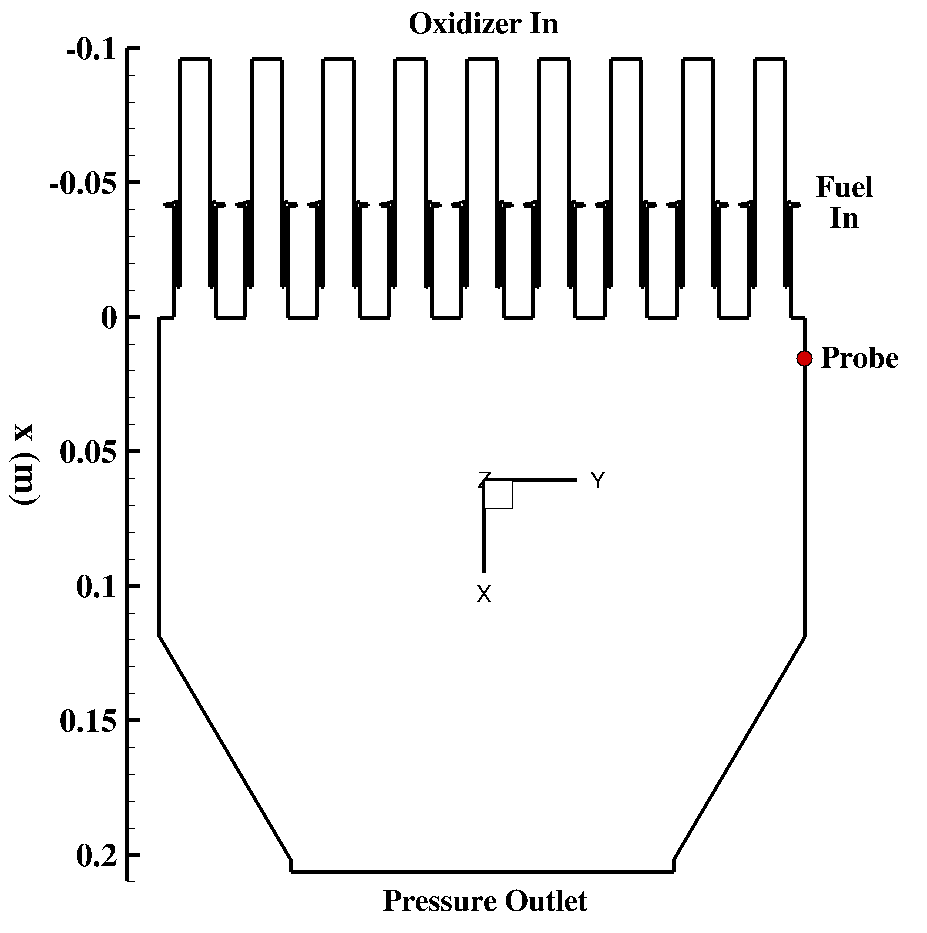
\includegraphics[width=0.99\linewidth]{Chapters/HPROMResults/Images/nineElem/geom_xy.png}
		\caption{\label{fig:nineElemGeomXY}Nine-element combustor geometry, $x-y$ cutaway.}
	\end{minipage}
	\begin{minipage}{0.49\linewidth}
		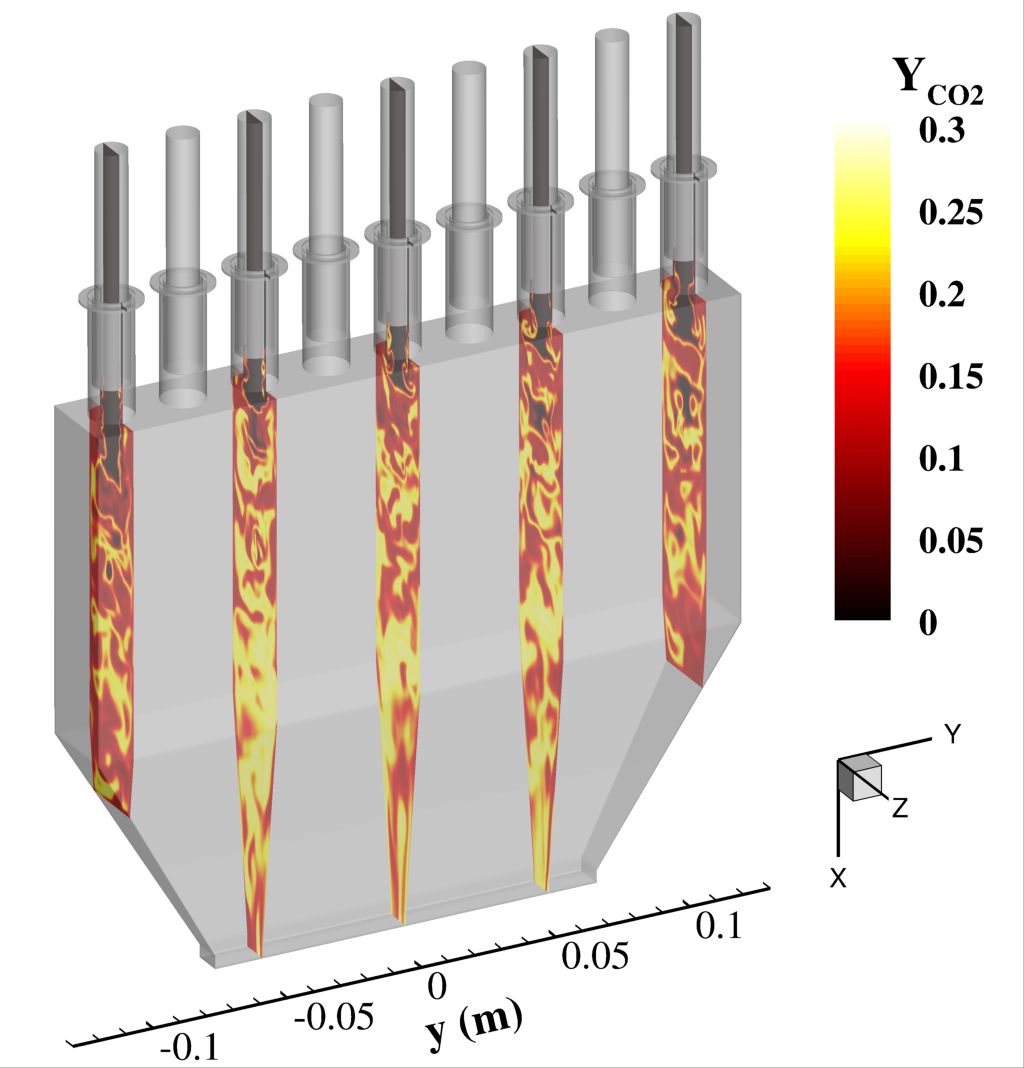
\includegraphics[width=0.99\linewidth]{Chapters/HPROMResults/Images/nineElem/geom_iso.png}
		\caption{\label{fig:nineElemGeomIso}Nine-element combustor geometry, isometric view, with $Y_{\text{CO}_2}$ $y-z$ slices at $\timeVar = 21.6$ ms.}
	\end{minipage}
\end{sidewaysfigure}

Mass flow rate boundary conditions are applied to the oxidizer and fuel inlets, though a single rate is enforced for the entire oxidizer inlet area, while individual rates are enforced for each fuel inlet. Adiabatic, no-slip wall conditions are enforced at all walls. A fixed pressure outlet is enforced at the nozzle exit, specifying an exit pressure of 101,325 Pa to model venting to atmosphere.

Reactions are modeled by a 12-species (plus inert nitrogen), 38-reaction finite-rate mechanism referred to as FFCMy-12, which is developed by Xu and Wang~\cite{Wang2018,Xu2018} as a reduced mechanism of the larger FFCM-1 mechanism~\cite{ffcm1} tailored for combustion of methane and oxygen in rocket combustors. As mentioned in Section~\ref{sec:finiterate}, this mechanism includes third-body low-pressure corrections of the Hinshelwood~\cite{Hinshelwood1926} and Troe~\cite{Gilbert1983} forms. This mechanism has been utilized previously in the simulation of traditional liquid rocket engines~\cite{Harvazinski2020,Harvazinski2021} as well as rotating detonation engines~\cite{Prakash2021,Batista2021}. The fluid is treated as a thermally-perfect gas, and thermodynamic and transport properties are computed by the empirical fit models described in Section~\ref{subsec:gasModels}. Subgrid dissipation is modeled via the Nicoud $\sigma$-model described in Section~\ref{subsec:subgrid}.

The computational mesh is composed of 14,387,292 hexahedral cells, resulting in a total full-order dimension of $\numDOF = 244,583,964$. To the best of the author's knowledge, this represents the largest case examined for PROMs of unsteady fluid flows, and also accounts for a significant increase in modeling complexity relative to comparable studies of aerodynamics problems.

\begin{figure}
	\begin{minipage}{0.49\linewidth}
		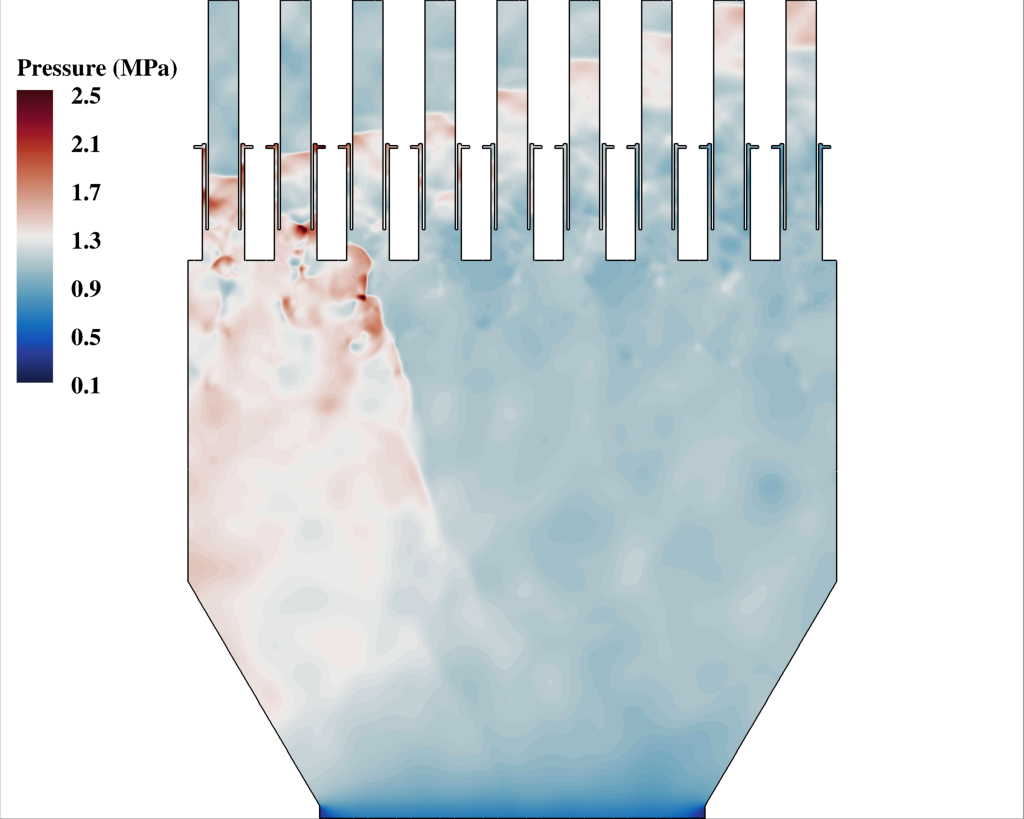
\includegraphics[width=0.99\linewidth,trim={0.5em 0em 6cm 0em},clip]{Chapters/HPROMResults/Images/nineElem/example_snaps/example_pressure_z.png}
	\end{minipage}
	\begin{minipage}{0.49\linewidth}
		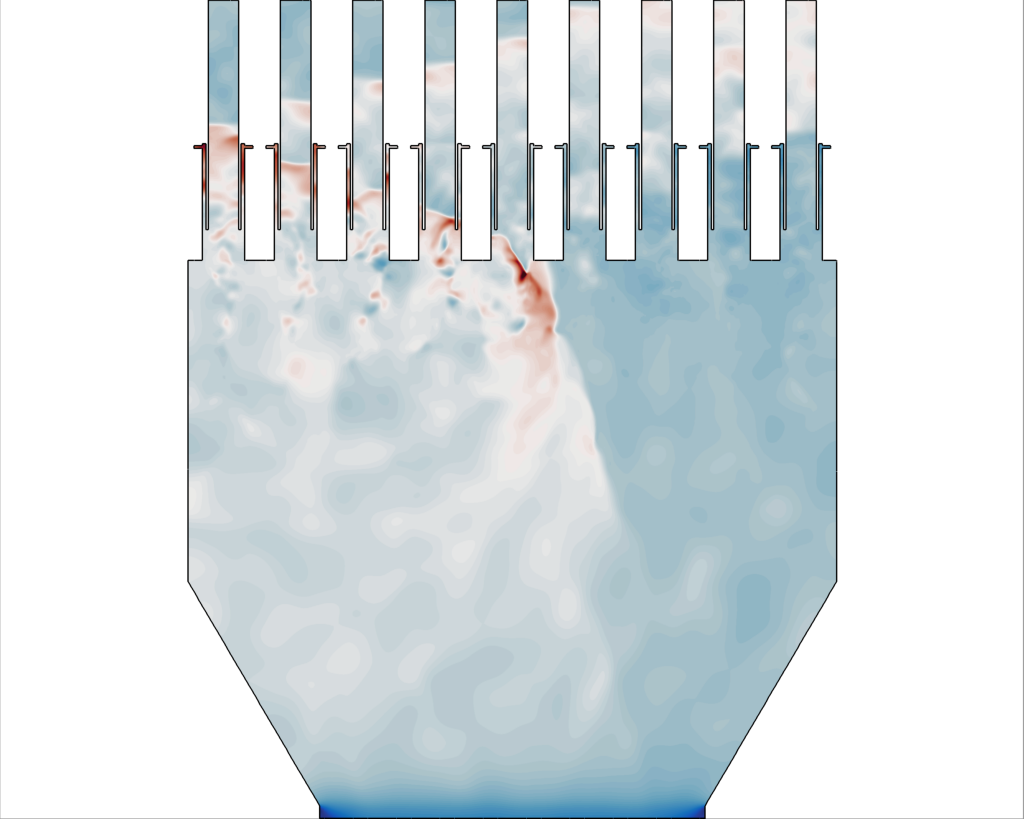
\includegraphics[width=0.99\linewidth,trim={6cm 0em 0.5em 0em},clip]{Chapters/HPROMResults/Images/nineElem/example_snaps/example_pressure_z_217000.png}
	\end{minipage}

	\begin{minipage}{0.49\linewidth}
		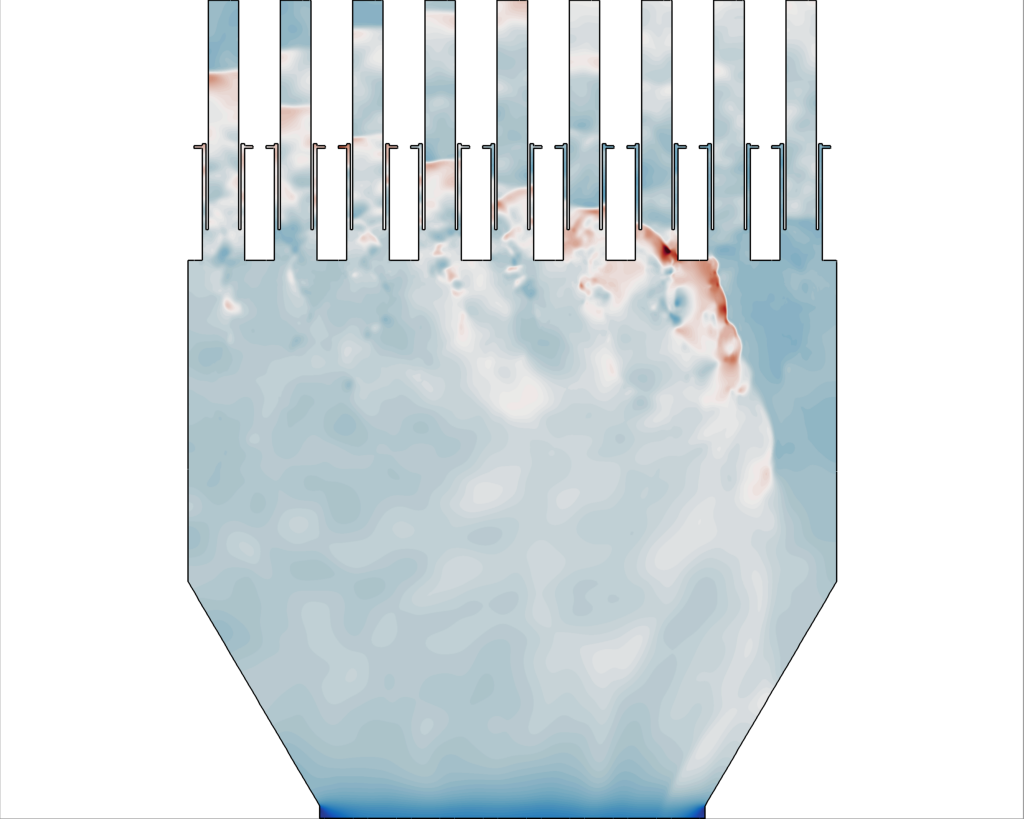
\includegraphics[width=0.99\linewidth,trim={0.5em 0em 6cm 0em},clip]{Chapters/HPROMResults/Images/nineElem/example_snaps/example_pressure_z_217500.png}
	\end{minipage}
	\begin{minipage}{0.49\linewidth}
		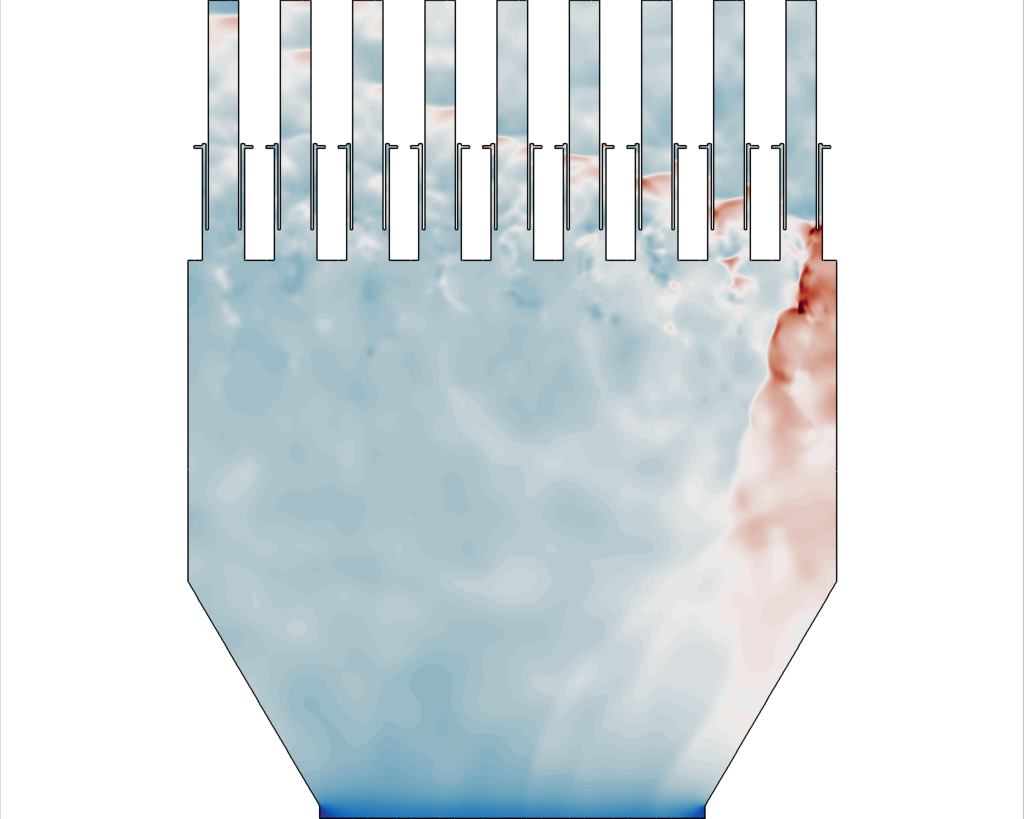
\includegraphics[width=0.99\linewidth,trim={6cm 0em 0.5em 0em},clip]{Chapters/HPROMResults/Images/nineElem/example_snaps/example_pressure_z_218000.png}
	\end{minipage}
	\caption{\label{fig:nineElemFOMPressure}FOM pressure slices for $x-y$ plane slice at $\timeVar = $ 21.65 (top left), 21.7 (top right), 21.75 (bottom left) and 21.8 (bottom right) ms.}
\end{figure}

\begin{figure}
	\begin{minipage}{0.49\linewidth}
		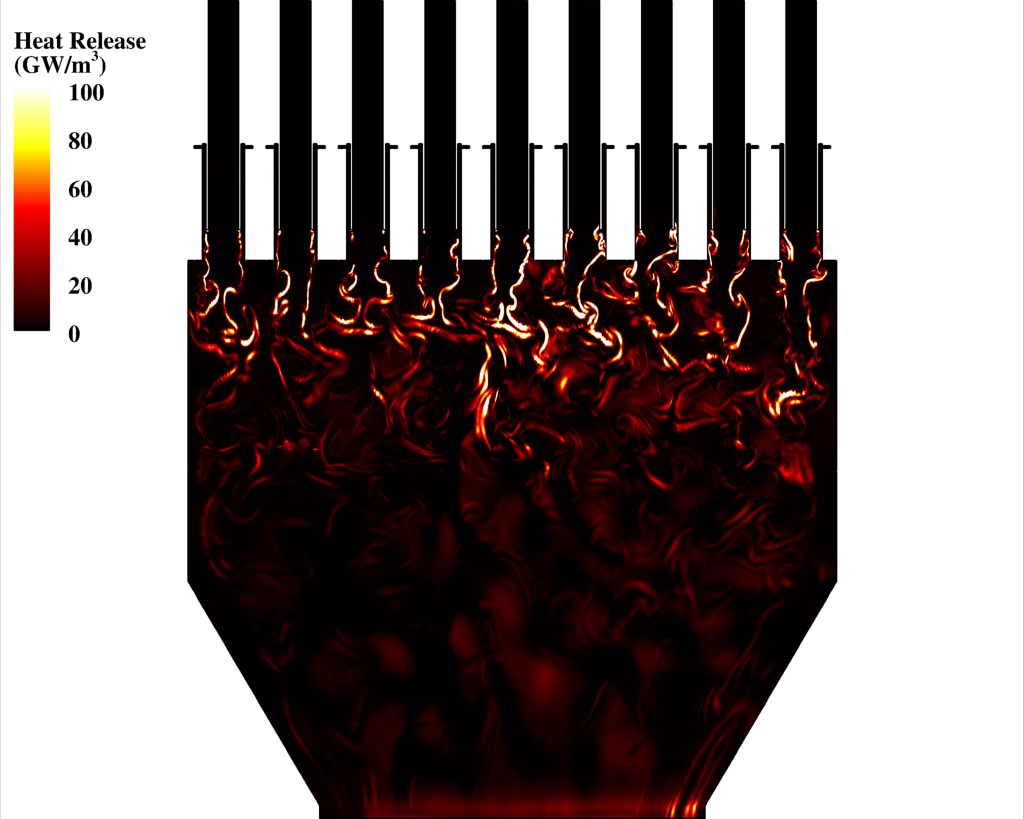
\includegraphics[width=0.99\linewidth,trim={0.5em 0em 6cm 0em},clip]{Chapters/HPROMResults/Images/nineElem/example_snaps/example_heat_z.png}
	\end{minipage}
	\begin{minipage}{0.49\linewidth}
		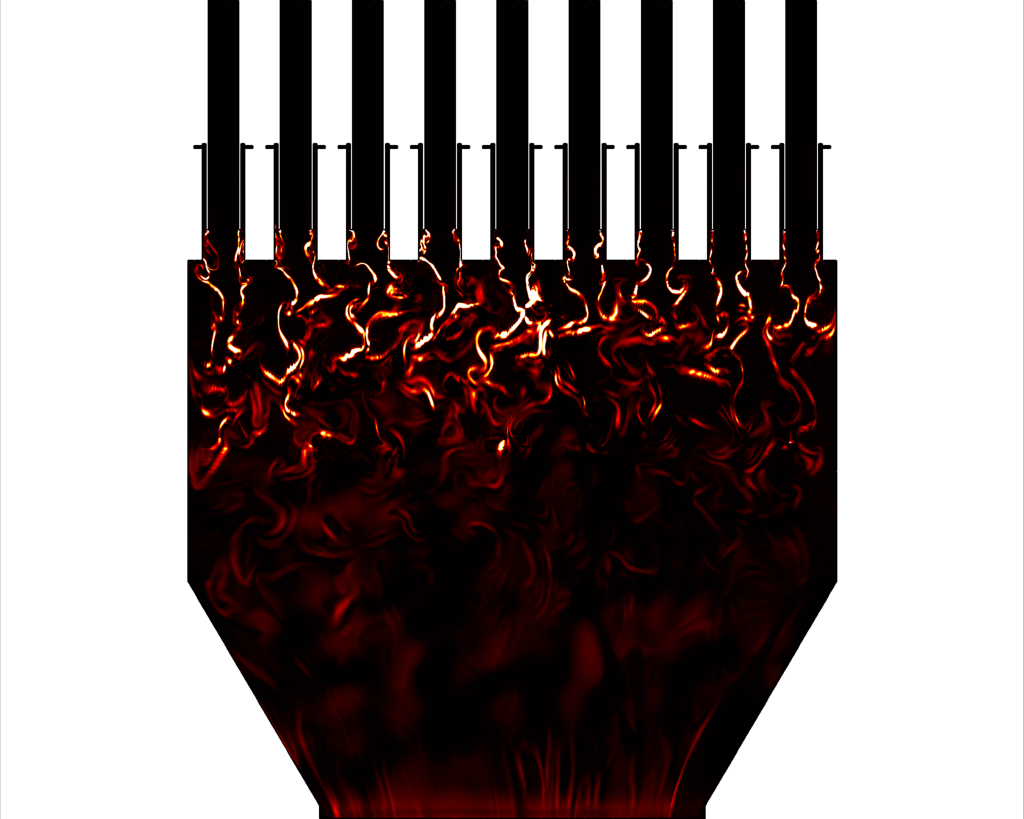
\includegraphics[width=0.99\linewidth,trim={6cm 0em 0.5em 0em},clip]{Chapters/HPROMResults/Images/nineElem/example_snaps/example_heat_z_217000.png}
	\end{minipage}

	\begin{minipage}{0.49\linewidth}
		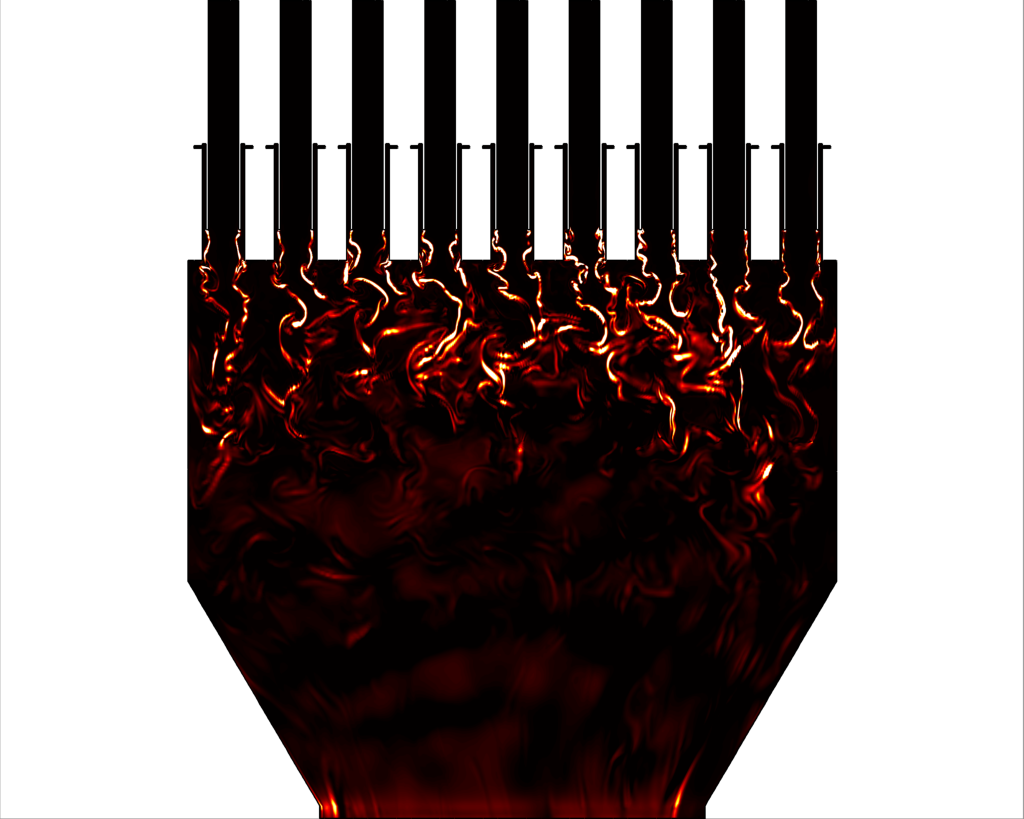
\includegraphics[width=0.99\linewidth,trim={0.5em 0em 6cm 0em},clip]{Chapters/HPROMResults/Images/nineElem/example_snaps/example_heat_z_217500.png}
	\end{minipage}
	\begin{minipage}{0.49\linewidth}
		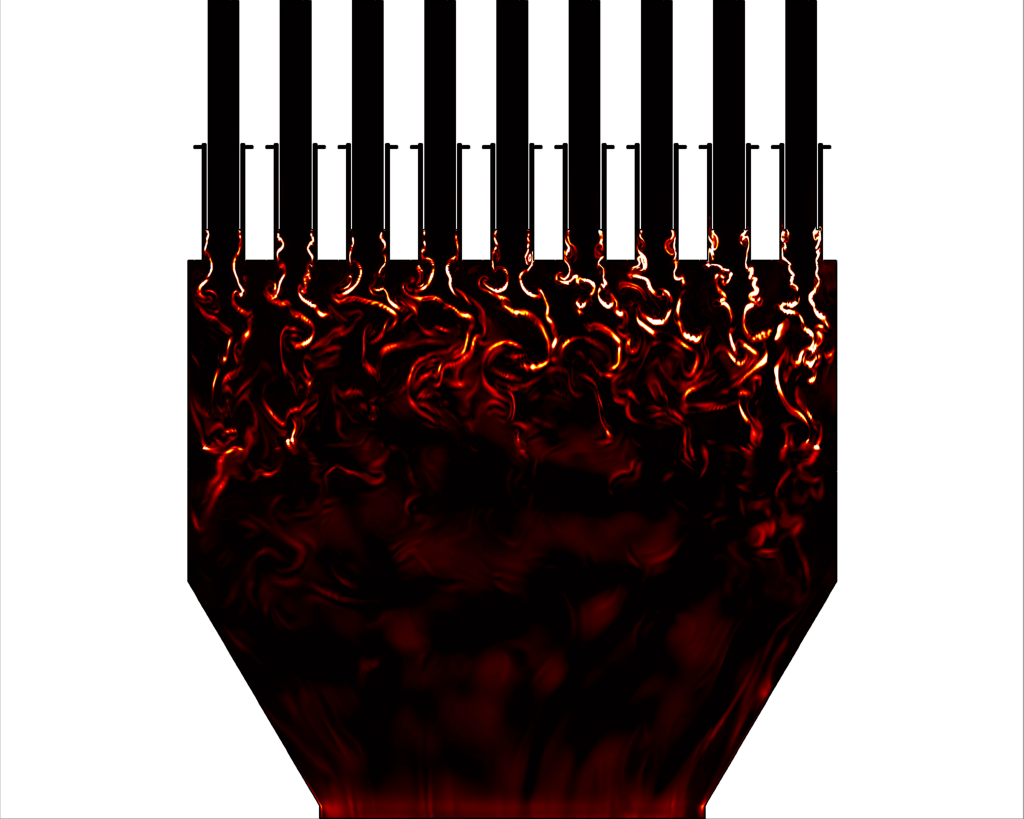
\includegraphics[width=0.99\linewidth,trim={6cm 0em 0.5em 0em},clip]{Chapters/HPROMResults/Images/nineElem/example_snaps/example_heat_z_218000.png}
	\end{minipage}
	\caption{\label{fig:nineElemFOMHeat}FOM heat release slices for $x-y$ plane slice at $\timeVar = $ 21.65 (top left), 21.7 (top right), 21.75 (bottom left) and 21.8 (bottom right) ms.}
\end{figure}

The FOM is initialized as follows. The entire domain is initialized with zero velocity and 1.138 MPa pressure. The oxidizer posts and propellant injection ports (excluding the fuel annuli) are initialized with 96.5\% oxygen and 3.5\% water vapor at 636 K. The fuel annuli are initialized with 100\% methane at 287.6 K. The combustion chamber is initialized with hot products (44\% water vapor and 56\% carbon dioxide) at 2,000 K. The physical time step size is $\dt = 0.1 \mu$s, and the FOM is first run for 216,000 steps (21.6 ms) to allow the transverse instability to initiate and for the flow to become statistically stationary. The instability is visualized in Fig.~\ref{fig:nineElemFOMPressure}, where a high-pressure wave traverses the width of the combustion chamber (reflecting from the walls) over the course of approximately 0.195 ms. The pressure wave is accompanied by heightened local heat release, which can be seen in Fig.~\ref{fig:nineElemFOMHeat}.

\begin{figure}
	\centering
	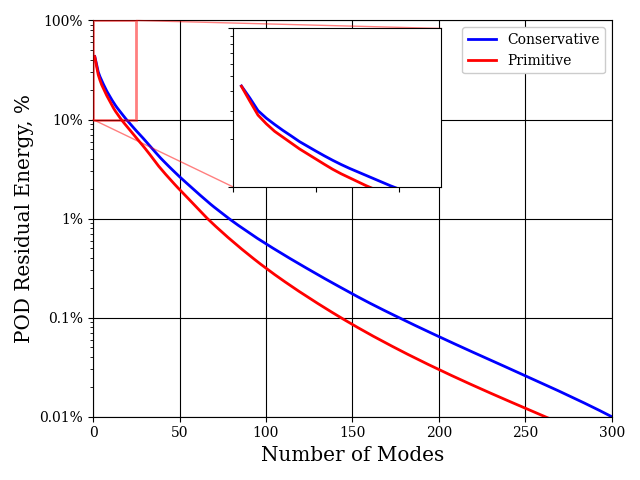
\includegraphics[width=0.8\linewidth]{Chapters/HPROMResults/Images/nineElem/nineElem_pod_energy.png}
	\caption{\label{fig:nineElemPODEnergy}POD residual energy decay for nine-element combustor conservative and primitive state datasets.}
\end{figure}

\begin{figure}
	\begin{minipage}{0.48\linewidth}
		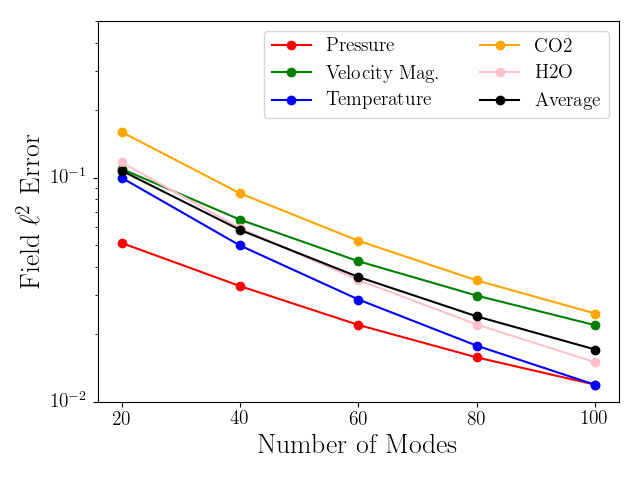
\includegraphics[width=0.99\linewidth,trim={0.5em 0.5em 0.5em 0.5em},clip]{Chapters/HPROMResults/Images/nineElem/projection_error_primitive.png}
		\caption{\label{fig:nineElemProjErrPrim}Primitive variables time-average projection error.}
	\end{minipage} \hspace{0.5em}
	\begin{minipage}{0.48\linewidth}
		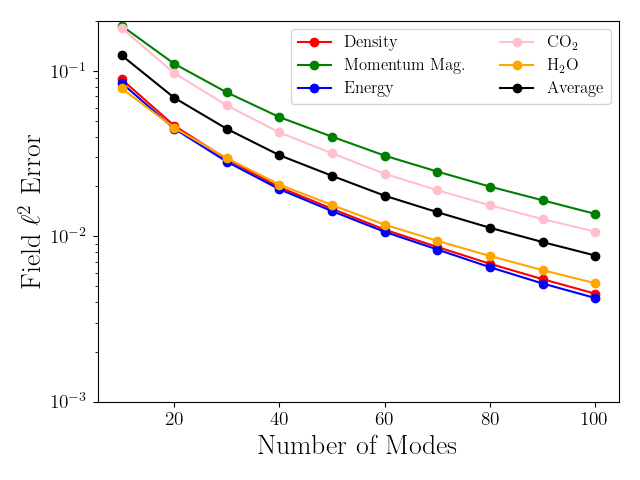
\includegraphics[width=0.99\linewidth,trim={0.5em 0.5em 0.5em 0.5em},clip]{Chapters/HPROMResults/Images/nineElem/projection_error_conservative.png}
		\caption{\label{fig:nineElemProjErrCons}Conservative variables time-average projection error.}
	\end{minipage}
\end{figure}

Starting at $\timeVar = 21.6$ ms, snapshots of the primitive and conservative states are collected at every time step until $\timeVar = 21.8$, resulting in 2,001 snapshots (including $\stateVec(\timeVar = 21.5 \text{ms})$). This window captures one complete traversal of the high-pressure wave along the width of the combustor. The POD residual energy decay is shown in Fig.~\ref{fig:nineElemPODEnergy}. Achieving 1\%, 0.1\%, and 0.01\% of the conservative state POD residual energy requires 53, 104, and 173 modes respectively. For the primitive state, this requires 35, 76, and 141 modes respectively. As with the truncated CVRC, this case exhibits an extremely slow POD residual energy decay characteristic of such a highly-nonlinear convection-dominated flow. The projection error of the primitive and conservative state datasets are shown in Figs.~\ref{fig:nineElemProjErrPrim} and~\ref{fig:nineElemProjErrCons} respectively. Interestingly, again the transverse and depth-wise velocity represent the largest sources of projection error. However, three of the most relevant transported scalars, carbon monoxide, carbon dioxide, and water vapor appear to induce less error than the fuel mixture fraction and progress variable did in the CVRC case.

\subsection{Unsampled PROMs}

Unsampled PROM accuracy is now investigated. Again, only MP-LSVT PROMs are examined, as Galerkin and LSPG PROMs were categorically unstable. This result is hardly surprising due to the extreme stiffness arising from the more detailed reaction mechanism. Results are evaluated for three time step values, $\dt \in \{2.5, \; 5, \; 10\} \times \dtFOM$, and primitive variable trial basis dimensions $\numPrimModes \in \{25, \; 50, \; 75, \; 100\}$. 

\begin{figure}
	\begin{minipage}{0.49\linewidth}
		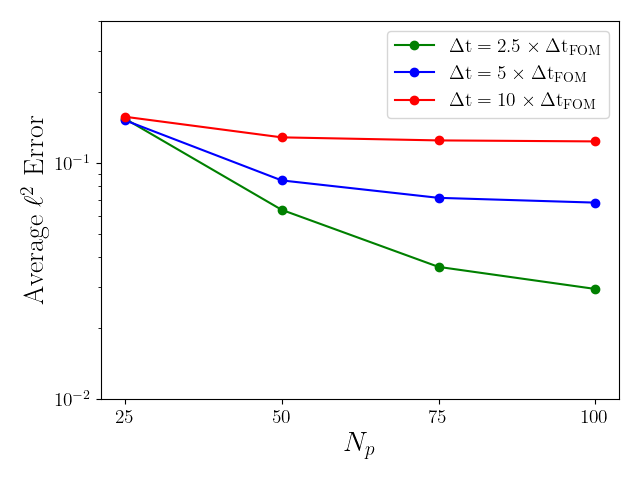
\includegraphics[width=0.99\linewidth]{Chapters/HPROMResults/Images/nineElem/unsampled/unsampled_avg_mode_Average_errorRaw.png}
		\caption{\label{fig:nineElemUnsampledError}Nine-element combustor unsampled PROM time-average error, various $\dt$.}
	\end{minipage}
	\begin{minipage}{0.49\linewidth}
		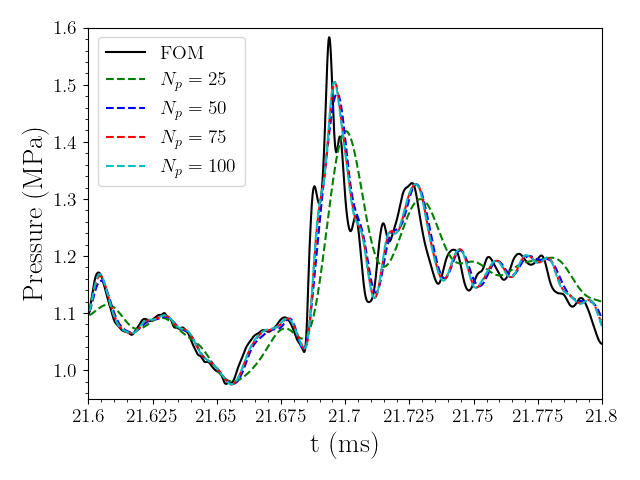
\includegraphics[width=0.99\linewidth]{Chapters/HPROMResults/Images/nineElem/unsampled/pressure_probe_unsampled_modes.png}
		\caption{\label{fig:nineElemUnsampledProbe}Nine-element combustor unsampled PROM pressure probe measurements, $\dt = 5 \times \dtFOM$, various $\numPrimModes$}
	\end{minipage}
\end{figure}

For results presented in this and the following section, average error is not computed across all primitive field variables, as this quantity appears exceptionally high even for large $\numPrimModes$. This is entirely due to deviations in chemical intermediates, such as monatomic species (H, O) and radicals (CH$_3$, OH, HO$_2$), which are extremely sensitive to small changes in reactant and other intermediate species fields. Although one may argue that the accuracy of reconstructing the reactant and final product fields is of primary concern, incorrect estimates of reaction intermediates undoubtedly degrades overall performance (particularly in predictions of unsteady heat release rates). Ignoring intermediate species, averages are computed over the primary flow field variables (pressure, velocity, and temperature) and primary chemical species (CH$_4$, O$_2$, H$_2$O, CO, CO$_2$). Figure~\ref{fig:nineElemUnsampledError}

\begin{figure}
	{\begin{minipage}{0.32\linewidth}
		\includegraphics[width=0.99\linewidth,trim={0.5em 0.5em 15.0em 0.5em},clip]{Chapters/HPROMResults/Images/nineElem/unsampled/fom_pressure_z.png}
	\end{minipage}
	\begin{minipage}{0.32\linewidth}
		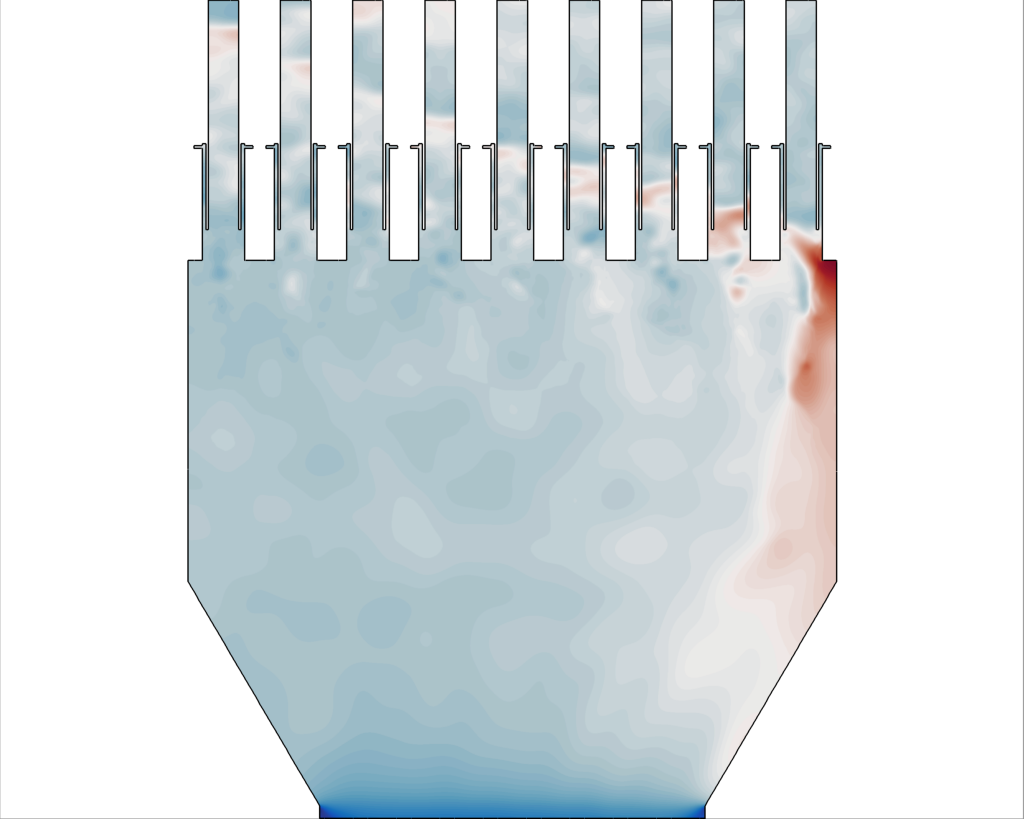
\includegraphics[width=0.99\linewidth,trim={0.5em 0.5em 15.0em 0.5em},clip]{Chapters/HPROMResults/Images/nineElem/unsampled/rom_k25_pressure_z.png}
	\end{minipage}
	\begin{minipage}{0.32\linewidth}
		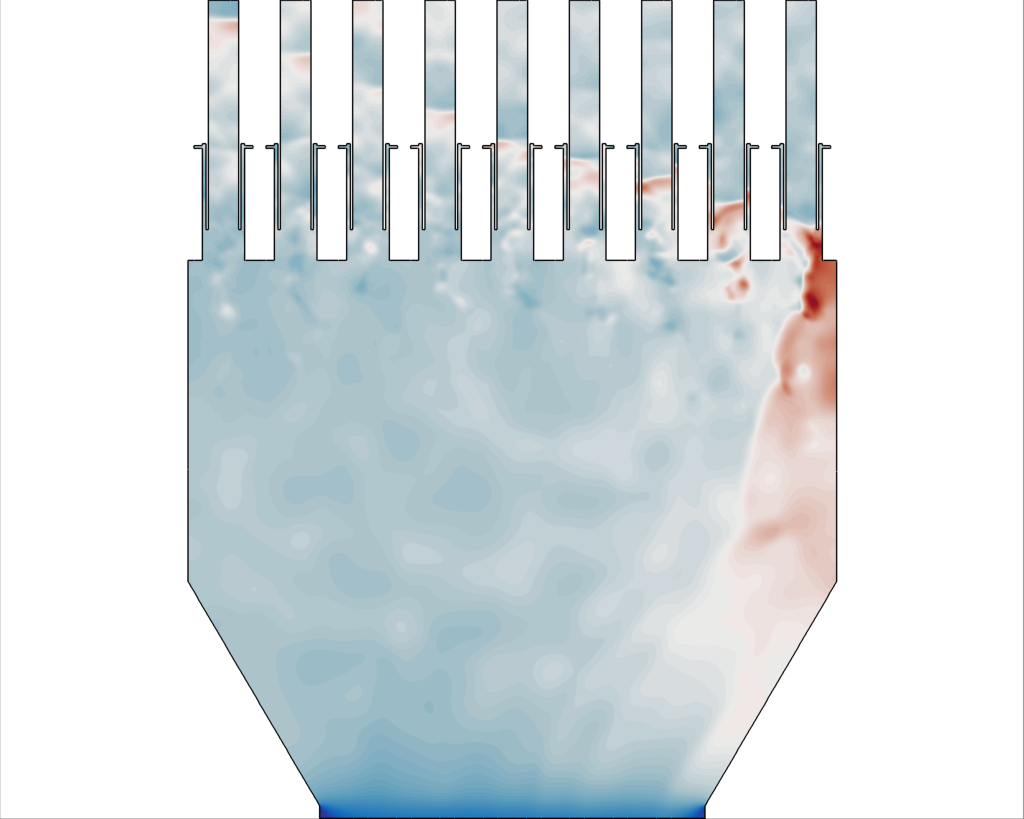
\includegraphics[width=0.99\linewidth,trim={0.5em 0.5em 15.0em 0.5em},clip]{Chapters/HPROMResults/Images/nineElem/unsampled/rom_k75_pressure_z.png}
	\end{minipage}
	\subcaption{\label{subfig:nineElemUnsampledPressure}Static pressure}}

	{\begin{minipage}{0.32\linewidth}
		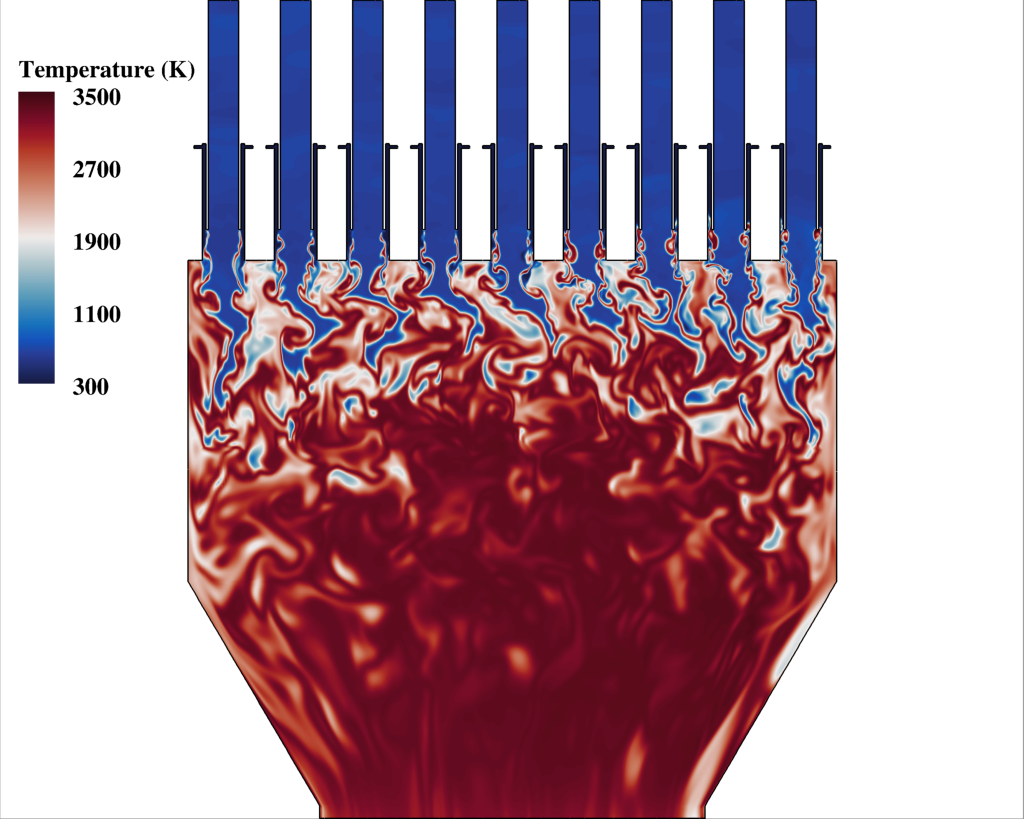
\includegraphics[width=0.99\linewidth,trim={0.5em 0.5em 15.0em 0.5em},clip]{Chapters/HPROMResults/Images/nineElem/unsampled/fom_temp_z.png}
	\end{minipage}
	\begin{minipage}{0.32\linewidth}
		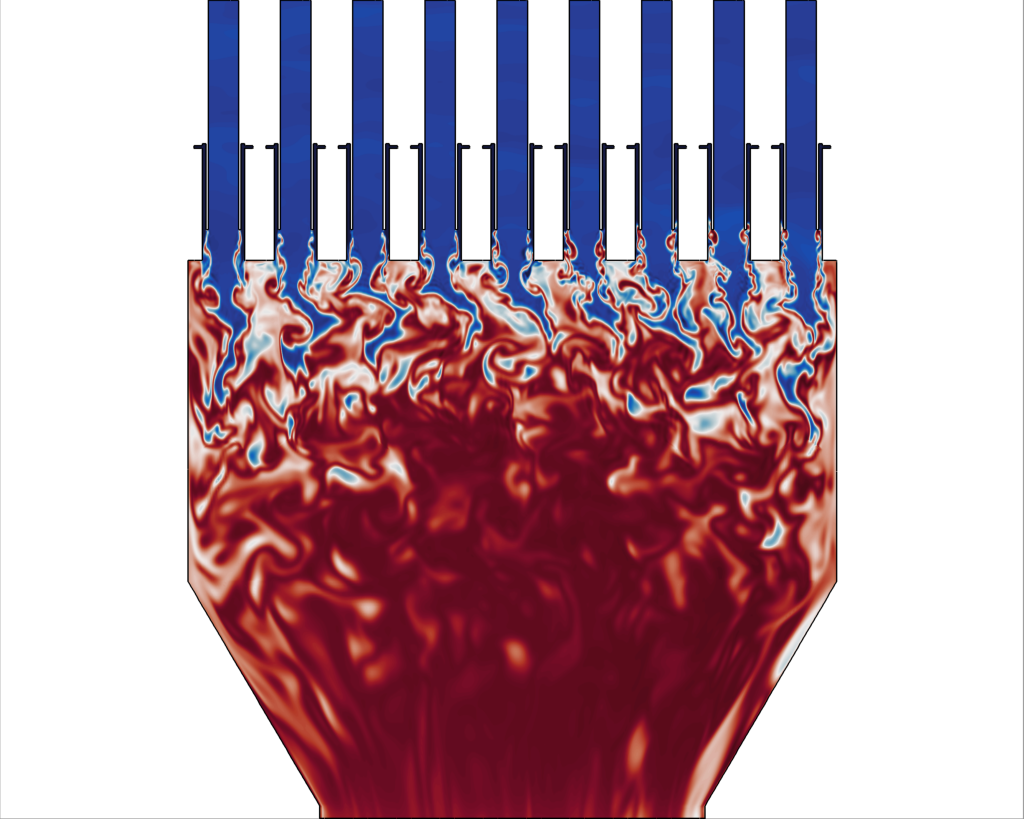
\includegraphics[width=0.99\linewidth,trim={0.5em 0.5em 15.0em 0.5em},clip]{Chapters/HPROMResults/Images/nineElem/unsampled/rom_k25_temp_z.png}
	\end{minipage}
	\begin{minipage}{0.32\linewidth}
		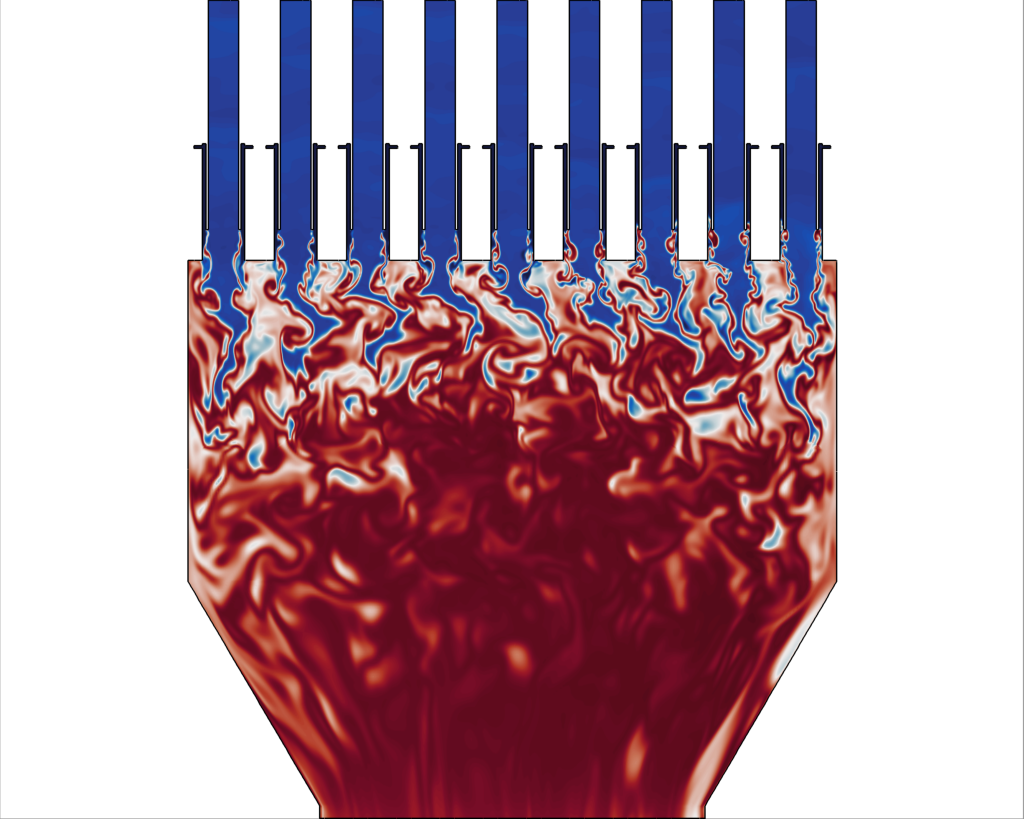
\includegraphics[width=0.99\linewidth,trim={0.5em 0.5em 15.0em 0.5em},clip]{Chapters/HPROMResults/Images/nineElem/unsampled/rom_k75_temp_z.png}
	\end{minipage}
	\subcaption{\label{subfig:nineElemUnsampledTemp}Temperature}}

	{\begin{minipage}{0.32\linewidth}
		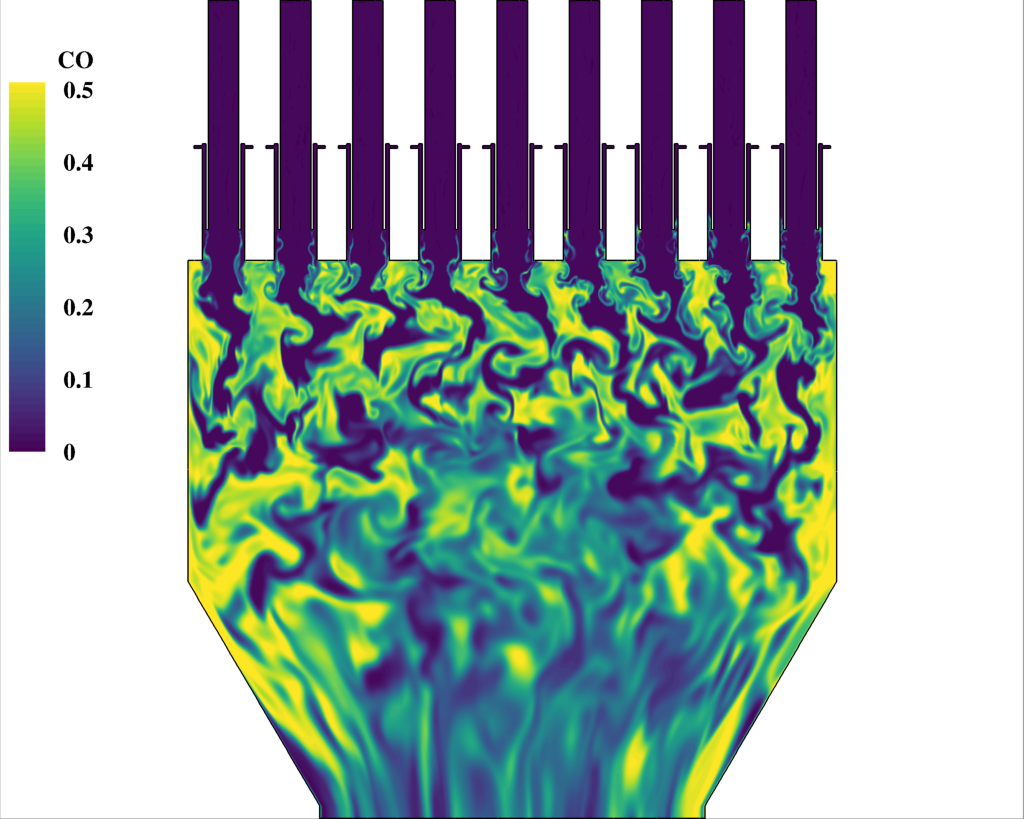
\includegraphics[width=0.99\linewidth,trim={0.5em 0.5em 15.0em 0.5em},clip]{Chapters/HPROMResults/Images/nineElem/unsampled/fom_co_z.png}
	\end{minipage}
	\begin{minipage}{0.32\linewidth}
		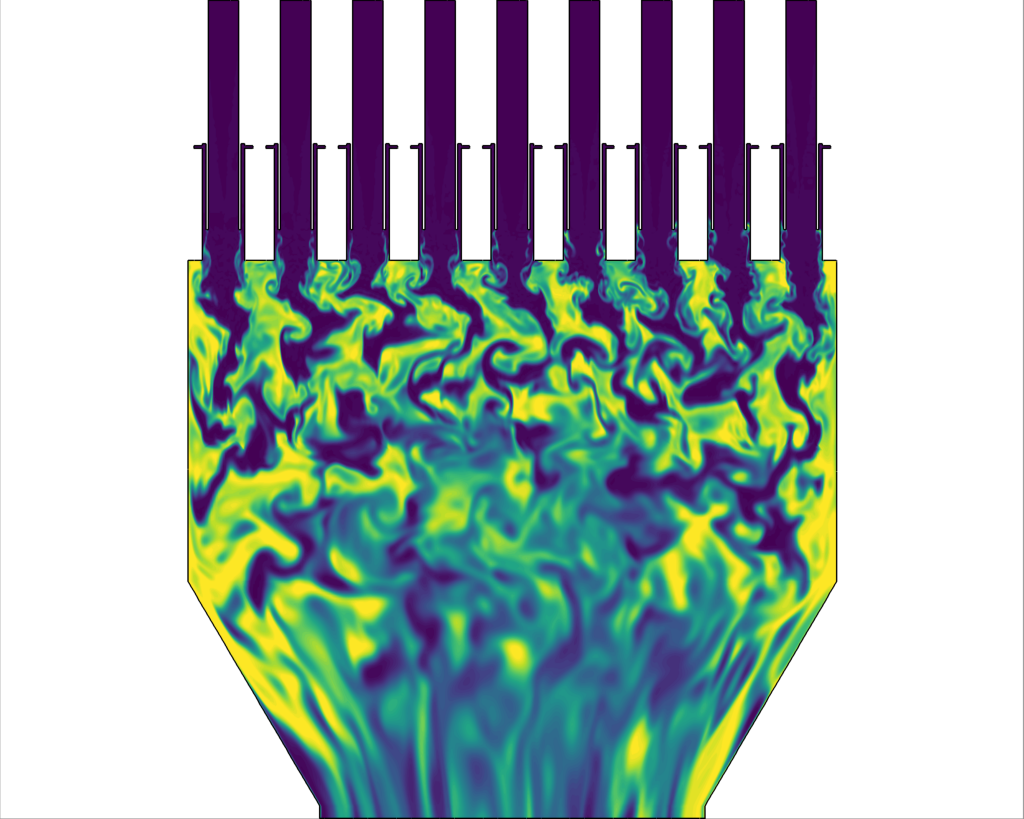
\includegraphics[width=0.99\linewidth,trim={0.5em 0.5em 15.0em 0.5em},clip]{Chapters/HPROMResults/Images/nineElem/unsampled/rom_k25_co_z.png}
	\end{minipage}
	\begin{minipage}{0.32\linewidth}
		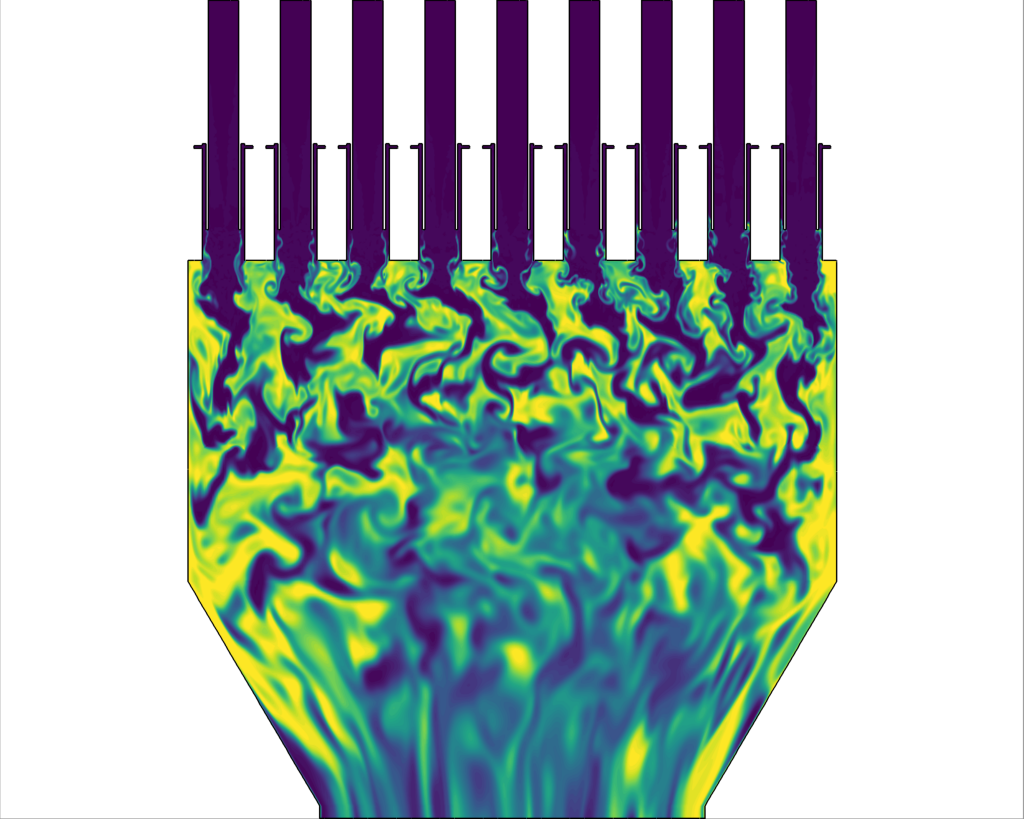
\includegraphics[width=0.99\linewidth,trim={0.5em 0.5em 15.0em 0.5em},clip]{Chapters/HPROMResults/Images/nineElem/unsampled/rom_k75_co_z.png}
	\end{minipage}
	\subcaption{\label{subfig:nineElemUnsampledCO}CO mass fraction}}

	\caption{\label{fig:nineElemUnsampledContours}Nine-element unsampled MP-LSVT PROM slices, $\timeVar = 21.8$ms, $\dt = 5 \times \dtFOM$. From left to right: FOM, $\numPrimModes=25$, $\numPrimModes=75$.}
\end{figure}

Examining several unsteady flow fields in Fig.~\ref{fig:nineElemUnsampledContours} provides visual insight into the unsteady evolution of the tightly-coupled acoustic, thermodynamic, and chemical interactions modeled by the PROM. Snapshots are taken from the end of the simulation period. Following similar trends observed for the CVRC, Fig.~\ref{subfig:nineElemUnsampledPressure} shows that enriching the trial basis tends to improve the reconstruction of sharp gradients, exemplified here by the high-pressure combustion instability. Such a trend is less immediately apparent for the temperature fields in Fig.~\ref{subfig:nineElemUnsampledTemp} and the carbon monoxide fields in Fig.~\ref{subfig:nineElemUnsampledCO}. Even at low $\numPrimModes$, the PROM is capable of reconstructing these unsteady states quite well. This can be reasonably attributed to the fact that transport of these fields is characterized a much slower time scale than that of the transverse pressure wave. As bulk advection has less of an effect on the temperature and transported scalar fields during the time window examined, one expects that the linear trial basis is better suited for modeling those fields.

The point-wise accuracy of reconstructing the high-pressure combustion instability is examined in the probe monitor results shown in Fig.~\ref{fig:nineElemUnsampledProbe}. As mentioned above, low trial basis dimensions ($\numPrimModes = 25$) tend to smear the pressure wave and generally fail to reconstruct the instantaneous probe measurements. Increasing the trial basis dimension to $\numPrimModes = 50$ improves on this measure, but enriching the trial basis further brings diminishing returns. Even increasing the basis dimension to $\numPrimModes = 100$ fails to capture much of the higher-frequency content or reproduce the maximum amplitude of the pressure signal. This implies a fundamental limitation of the linear trial basis, which struggles to recreate the complex interaction between the high-pressure transverse wave and the longitudinal reacting shear layers. However, given the extreme physical complexity and numerical stiffness of this problem, even these results are a testament to the robustness of the MP-LSVT method. 


\subsection{Hyper-reduced PROMs}

\begin{table}
	\centering
	\begin{tabular}{ lllllll }
	\toprule
	Sampling Rate (\%) & 0.025 & 0.05 & 0.1 & 0.25 & 0.5 & 1.0 \\
	\midrule
	Cores & 44 & 88 & 132 & 308 & 572 & 1100 \\
	Cells/core (approx.) & 82 & 82 & 109 & 117 & 126 & 131 \\
	\bottomrule
	\end{tabular}
	\caption{\label{tab:nineElemSampProcs}Partitioning for nine-element combustor HPROM sample meshes.}
\end{table}

Again, analyses for hyper-reduced MP-LSVT PROMs are repeated for the nine-element combustor. All results presented here use a physical time step of $\dt = 5 \times \dtFOM$, as well as a trial basis dimension of $\numPrimModes = 75$. The gappy POD regressors are constructed from the conservative field data. The investigation for this case is slightly more limited in scope than those presented for the cavity flow and truncated CVRC cases due to the significantly higher computational cost. As such, results exploring the effects of the sampling rate and gappy POD regressor dimension are coarser. Further, as will be shown shortly, only random sampling was capable of generating stable HPROM simulations; the partitioning data provided in Table~\ref{tab:nineElemSampProcs} reflects this fact, as random sampling requires an exceptionally large number of auxiliary cells. The seemingly low cells/core counts is simply an indicator of the need for more cores to complete calculations on these large meshes in a timely fashion. Example isosurfaces of the sample mesh for random and eigenvector-based sampling are presented in Fig.~\ref{fig:nineElemIblankIso} illustrate this fact well, showing that the greedy method generates an extremely compact sample mesh centered on the reacting shear layer of each injector, while the randomly-sampled mesh is distributed throughout the domain.

\begin{figure}
	\begin{minipage}{0.49\linewidth}
		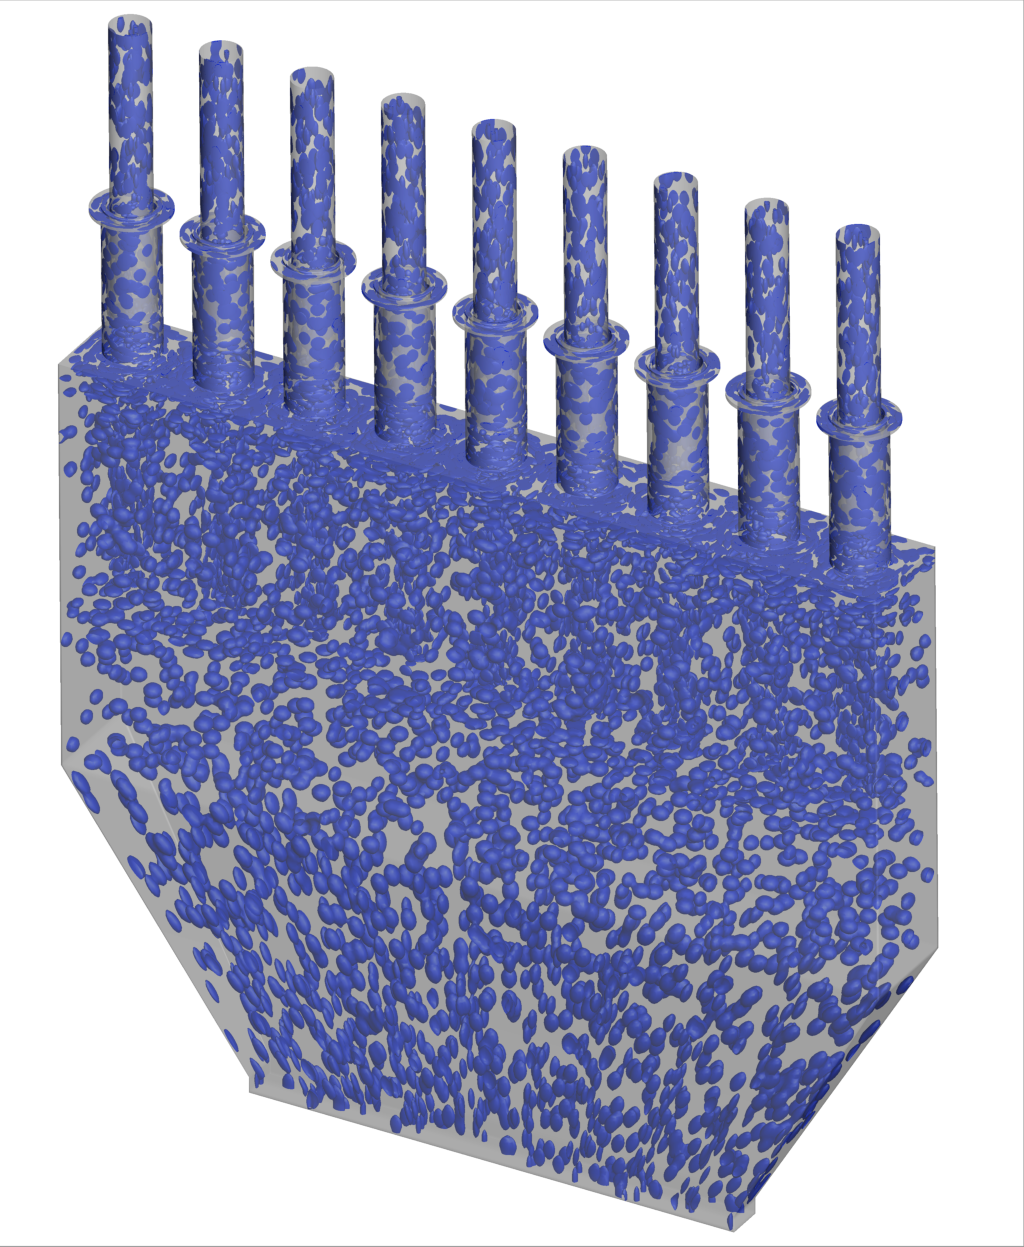
\includegraphics[width=0.99\linewidth,trim={0.3em 0.3em 0.3em 0.3em},clip]{Chapters/HPROMResults/Images/nineElem/deim/iblank/random_iblank_iso.png}
	\end{minipage}
	\begin{minipage}{0.49\linewidth}
		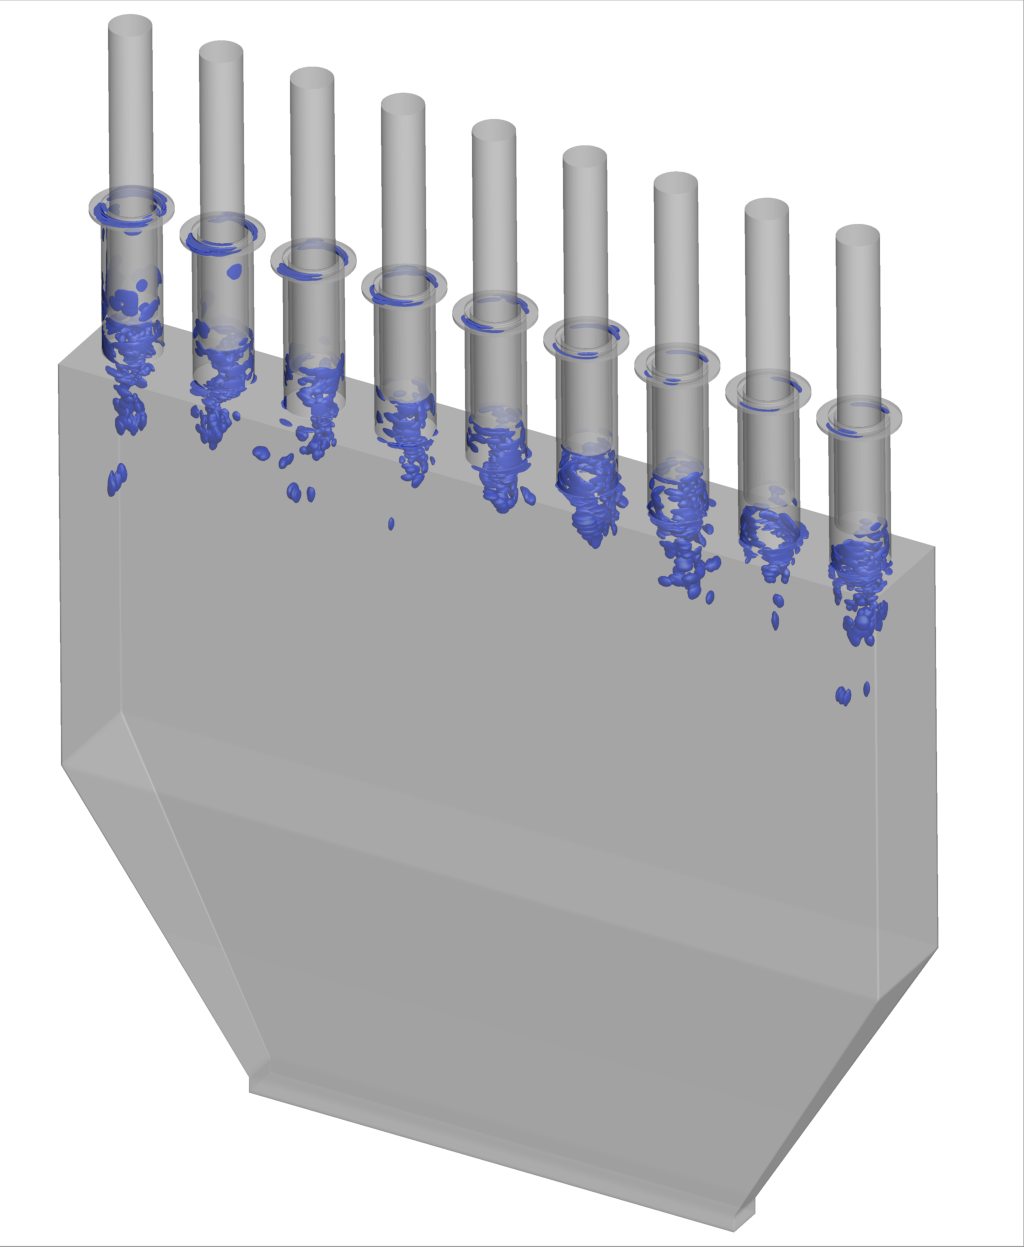
\includegraphics[width=0.99\linewidth,trim={0.3em 0.3em 0.3em 0.3em},clip]{Chapters/HPROMResults/Images/nineElem/deim/iblank/eigenvec_iblank_iso.png}
	\end{minipage}
	\caption{\label{fig:nineElemIblankIso}Example nine-element combustor sample meshes for $\numSamps = 0.1\% \times \numDOF$, $\numResModes = 100$, with random sampling (left) and eigenvector-based sampling (right).}
\end{figure}

The poor performance of the eigenvector-based sampling algorithm is made immediately apparent in the pressure probe measurements displayed in Fig.~\ref{fig:nineElemDEIMProbeAlgo}. Even for $\numSamps = 0.1\% \times \numDOF$ (for which the algorithm performed quite well for the cavity and CVRC cases), the solution employing sample meshes computed via the eigenvector-based sampling almost immediately diverges and quickly becomes unstable. The same behavior is observed for sampling rates up to $\numSamps = 0.25\% \times \numDOF$, after which point the offline computational cost of computing the sample mesh becomes exorbitantly large ($>$20,000 core-hours). Comparatively, the random sampling algorithm requires negligible offline computational cost and is capable of producing a reasonable reconstruction of the unsteady pressure signal. Drawing attention again to the sample mesh visualization in Fig.~\ref{fig:nineElemIblankIso}, note that the eigenvector-based algorithm selects cells in tight clusters either at the fuel injection ports or in the mixing shear layer of each injector. Few cells are placed in the combustion chamber, where the high-pressure combustion instability occurs and is sustained by the high heat release of the completed reaction. In this context, it is not surprising that this greedy algorithm is incapable of modeling the traversal of the pressure wave across the width of the combustion chamber. Although not shown here, both variants of the GNAT sampling algorithm perform equally poorly (unsurprisingly, as those algorithms tend to cluster samples even more closely).  

\begin{figure}
	\begin{minipage}{0.49\linewidth}
		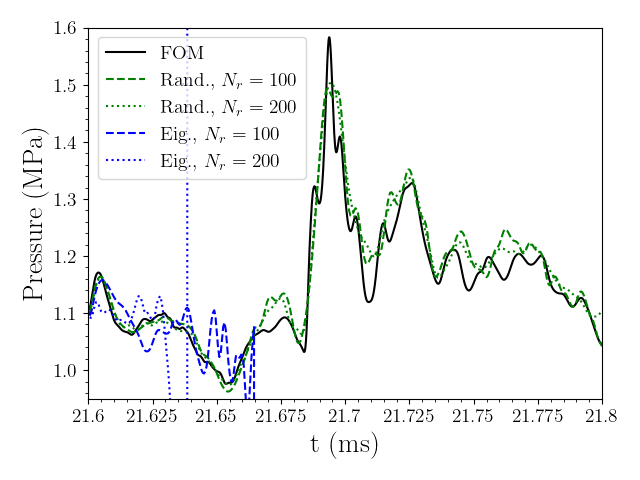
\includegraphics[width=0.99\linewidth]{Chapters/HPROMResults/Images/nineElem/deim/pressure_probe_deim_algs.png}
		\caption{\label{fig:nineElemDEIMProbeAlgo}Nine-element combustor HPPROM pressure probe measurements, $\numSamps = 0.1\% \times \numDOF$, various sampling algorithms and $\numResModes$.}
	\end{minipage}
	\begin{minipage}{0.49\linewidth}
		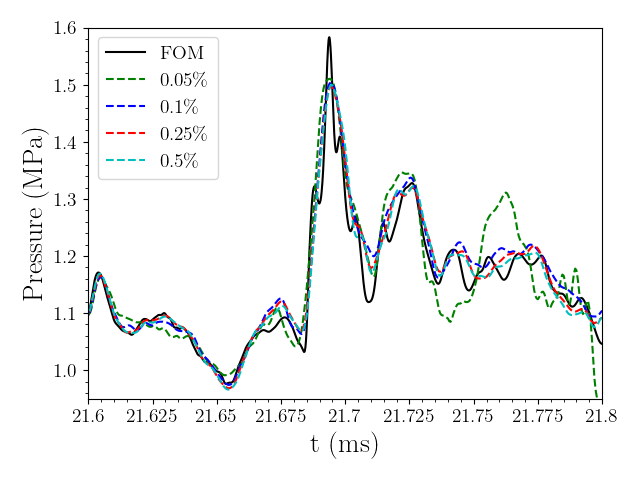
\includegraphics[width=0.99\linewidth]{Chapters/HPROMResults/Images/nineElem/deim/pressure_probe_deim_random_samp.png}
		\caption{\label{fig:nineElemDEIMProbeSamp}Nine-element combustor HPPROM pressure probe measurements, random sampling, $\numResModes = 200$, various $\numSamps$.}
	\end{minipage}
\end{figure}

On the one hand, this results is somewhat discouraging after the excellent performance of the eigenvector-based sampling algorithm for the cavity and CVRC cases. However, it also sheds light on the need for advanced hyper-reduction methods for problems which exhibit spatially-distributed convective phenomena (the transverse pressure wave), which may be tightly coupled to spatially-localized physics (propellant injection). As will be displayed in the following chapter, online trial basis and sample mesh adaptation proposes solutions to such problems, allowing the sample mesh to evolve with time and more accurately capture bulk advection effects. Such methods are not applied to this case, unfortunately, as the implementation of the underlying adaptation algorithms is not yet memory-scalable, and cannot solve adaptive ROM systems of such high dimensionality.

\begin{figure}
	{\begin{minipage}{0.32\linewidth}
		\includegraphics[width=0.99\linewidth,trim={0.5em 0.5em 15.0em 0.5em},clip]{Chapters/HPROMResults/Images/nineElem/deim/contours/fom_pressure_z.png}
	\end{minipage}
	\begin{minipage}{0.32\linewidth}
		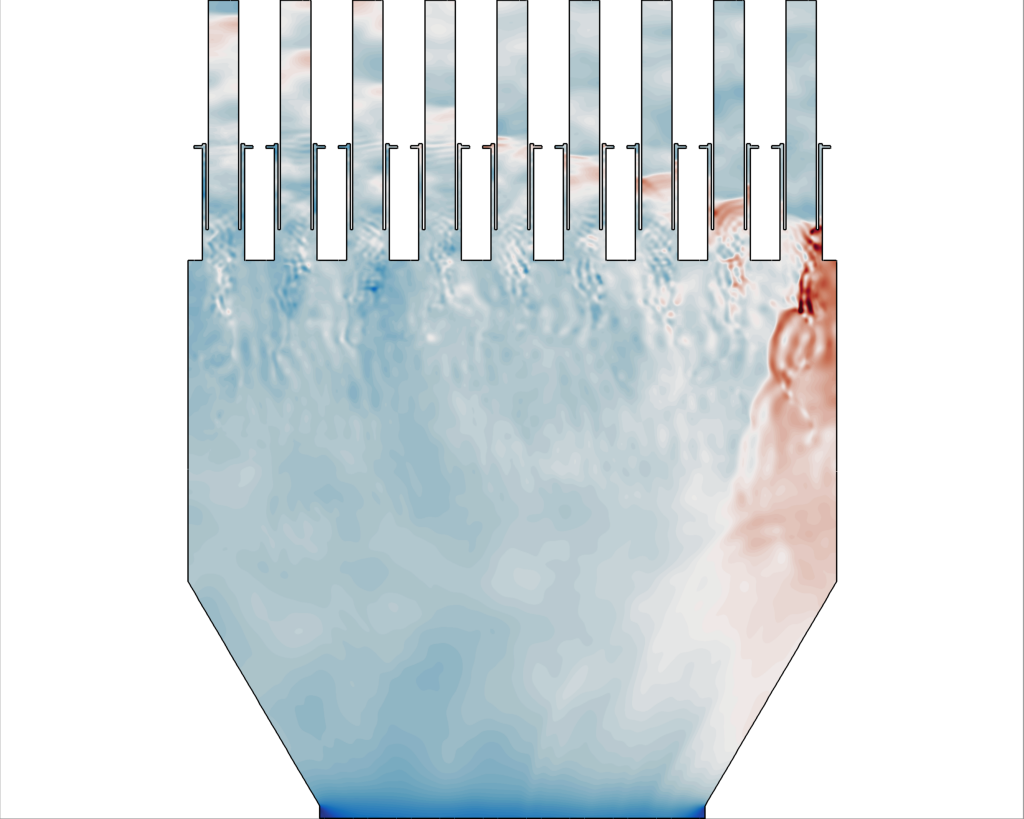
\includegraphics[width=0.99\linewidth,trim={0.5em 0.5em 15.0em 0.5em},clip]{Chapters/HPROMResults/Images/nineElem/deim/contours/deim_0p001_pressure_z.png}
	\end{minipage}
	\begin{minipage}{0.32\linewidth}
		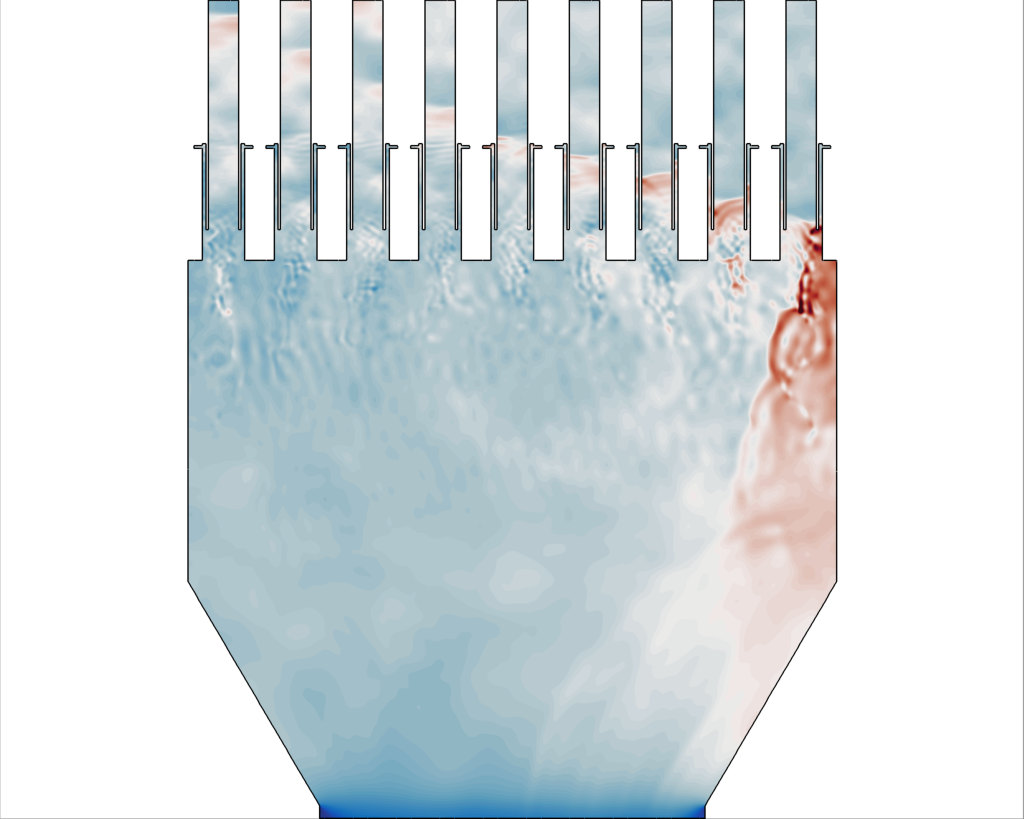
\includegraphics[width=0.99\linewidth,trim={0.5em 0.5em 15.0em 0.5em},clip]{Chapters/HPROMResults/Images/nineElem/deim/contours/deim_0p005_pressure_z.png}
	\end{minipage}
	\subcaption{\label{subfig:nineElemSampledPressure}Static pressure}}

	{\begin{minipage}{0.32\linewidth}
		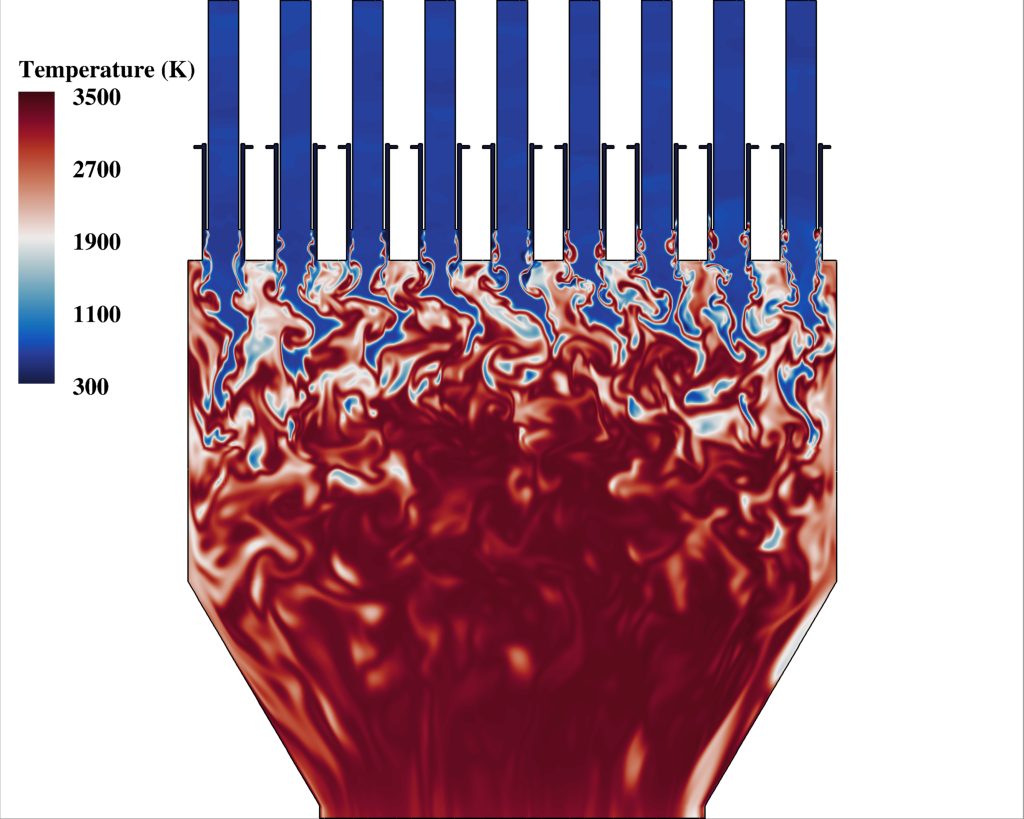
\includegraphics[width=0.99\linewidth,trim={0.5em 0.5em 15.0em 0.5em},clip]{Chapters/HPROMResults/Images/nineElem/deim/contours/fom_temp_z.png}
	\end{minipage}
	\begin{minipage}{0.32\linewidth}
		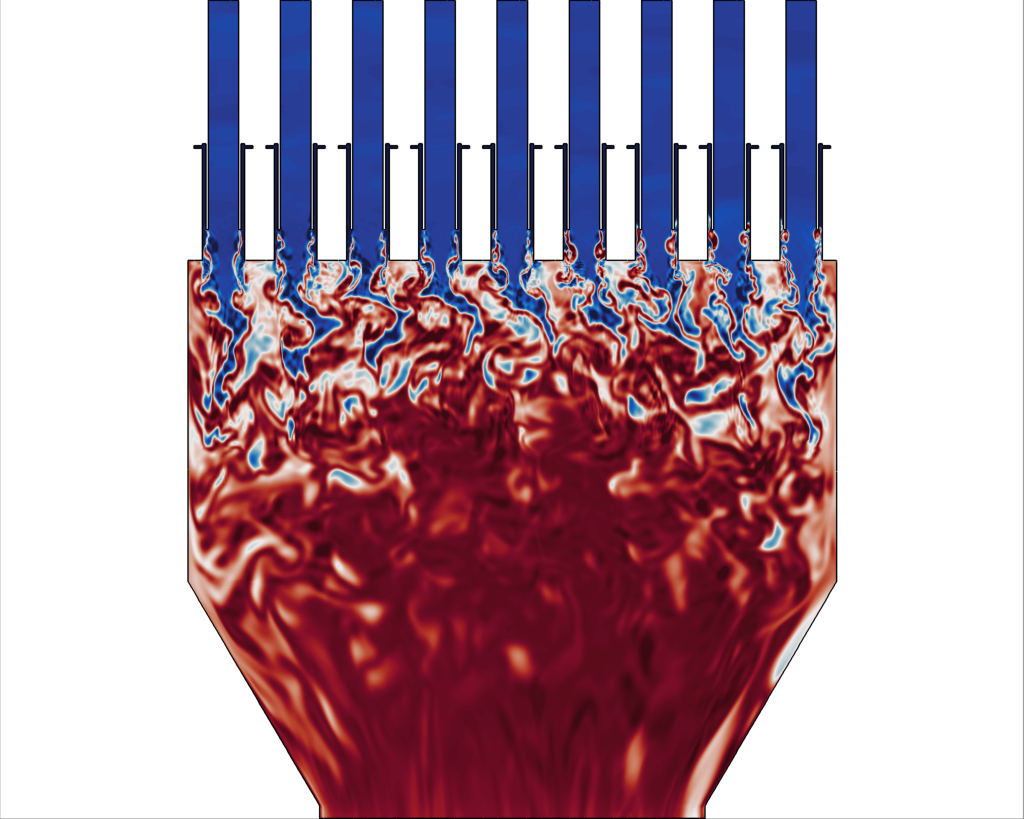
\includegraphics[width=0.99\linewidth,trim={0.5em 0.5em 15.0em 0.5em},clip]{Chapters/HPROMResults/Images/nineElem/deim/contours/deim_0p001_temp_z.png}
	\end{minipage}
	\begin{minipage}{0.32\linewidth}
		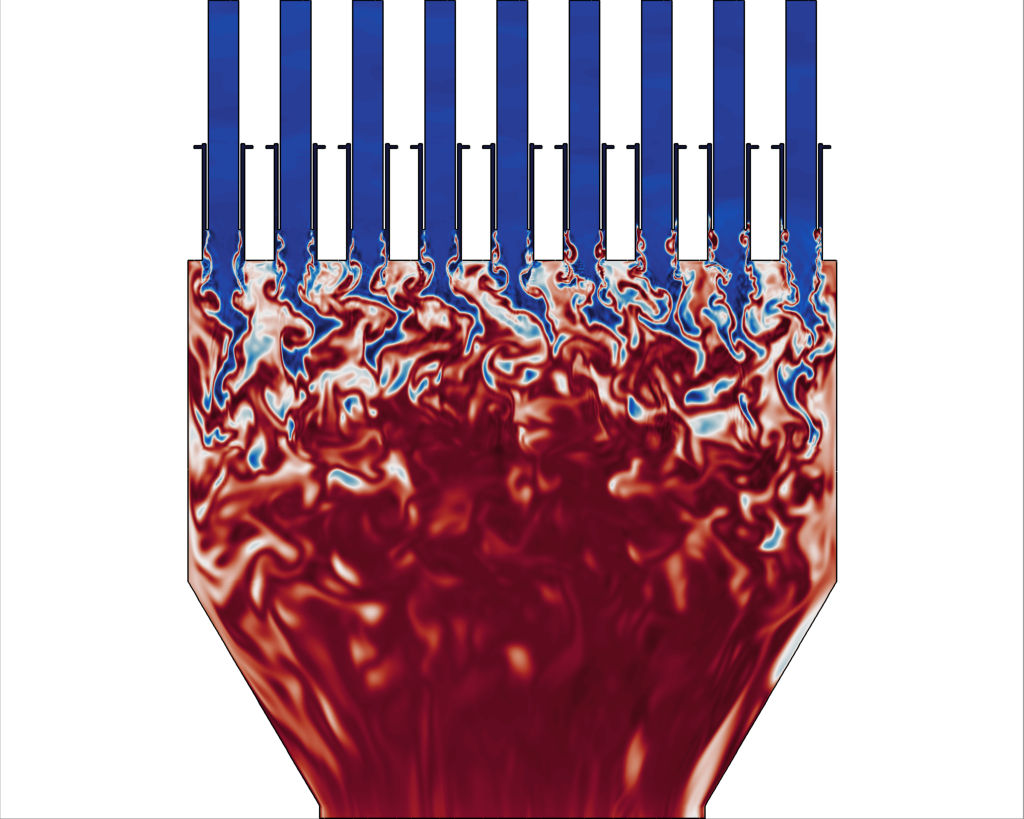
\includegraphics[width=0.99\linewidth,trim={0.5em 0.5em 15.0em 0.5em},clip]{Chapters/HPROMResults/Images/nineElem/deim/contours/deim_0p005_temp_z.png}
	\end{minipage}
	\subcaption{\label{subfig:nineElemSampledTemp}Temperature}}

	{\begin{minipage}{0.32\linewidth}
		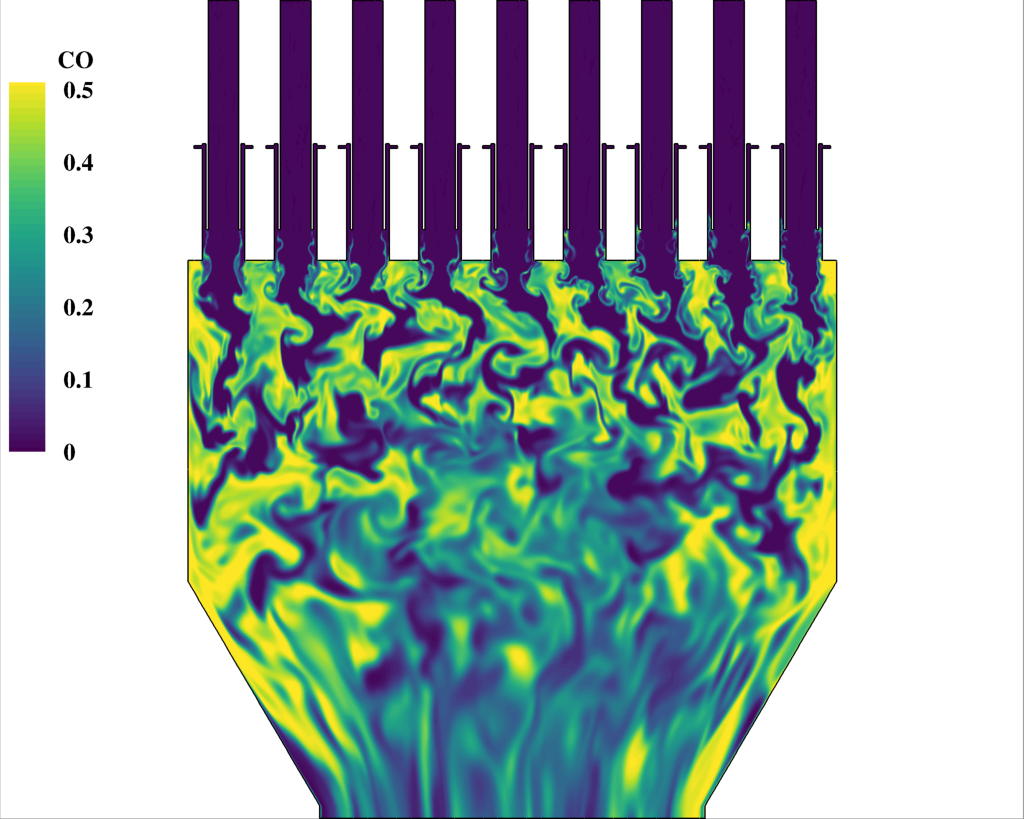
\includegraphics[width=0.99\linewidth,trim={0.5em 0.5em 15.0em 0.5em},clip]{Chapters/HPROMResults/Images/nineElem/deim/contours/fom_co_z.png}
	\end{minipage}
	\begin{minipage}{0.32\linewidth}
		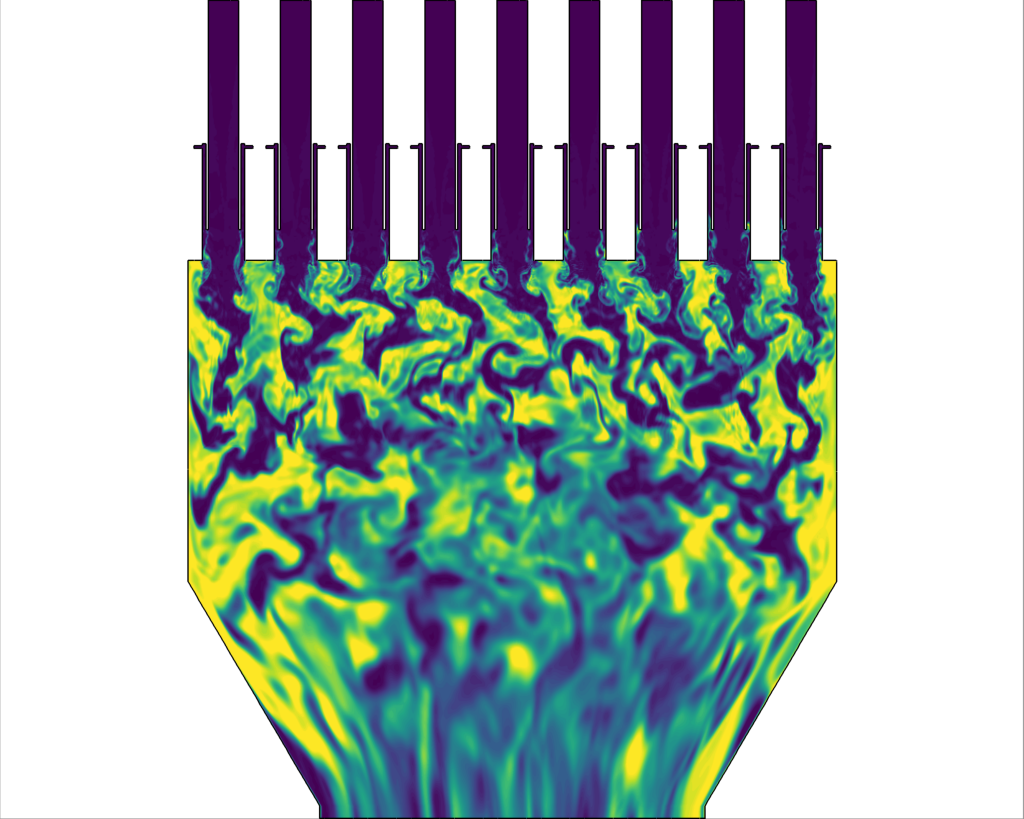
\includegraphics[width=0.99\linewidth,trim={0.5em 0.5em 15.0em 0.5em},clip]{Chapters/HPROMResults/Images/nineElem/deim/contours/deim_0p001_co_z.png}
	\end{minipage}
	\begin{minipage}{0.32\linewidth}
		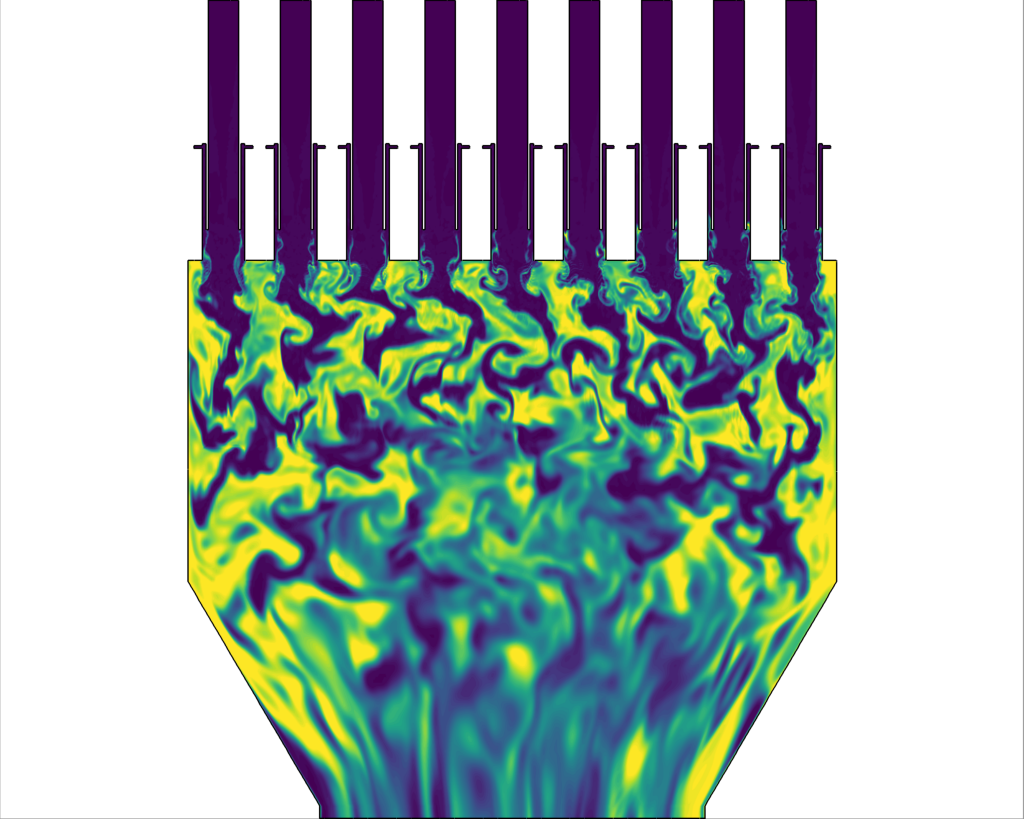
\includegraphics[width=0.99\linewidth,trim={0.5em 0.5em 15.0em 0.5em},clip]{Chapters/HPROMResults/Images/nineElem/deim/contours/deim_0p005_co_z.png}
	\end{minipage}
	\subcaption{\label{subfig:nineElemSampledCO}CO mass fraction}}

	\caption{\label{fig:nineElemDEIMContours}Nine-element HPROM slices, $\timeVar = 21.8$ms, $\numResModes = 200$, $\dt = 5 \times \dtFOM$. From left to right: FOM, $\numSamps = 0.1\% \times \numDOF$, $\numSamps = 0.5\% \times \numDOF$.}
\end{figure}

Despite the inadequate performance of the greedy sampling algorithms, the random sampling method is still capable of generating good results, even for a system of this complexity and size. Figure~\ref{fig:nineElemDEIMContours} displays several sample slices to this effect, showing HPROM results at the end of the simulation time window for $\numSamps \in \{0.1, \; 0.5 \}\% \times \numDOF$. Although the pressure field (Fig.~\ref{subfig:nineElemSampledPressure}) exhibits significant spurious oscillations near the injector face, the temperature (Fig.~\ref{subfig:nineElemSampledTemp}) and CO mass fraction (Fig.~\ref{subfig:nineElemUnsampledCO}) fields reconstruct those of the FOM with remarkable accuracy. The effect of the sampling rate is displayed via pressure monitor measurements in Fig.~\ref{fig:nineElemDEIMProbeSamp}: below $\numSamps = 0.1\% \times \numSamps$, the long-term accuracy of the solution begins to degrade noticeably, while increasing the sampling rate results in marginal improvement. Although the HPROMs appear incapable of capturing the full amplitude of the pressure wave, this may be attributed to the coarseness of the trial basis, as it was observed that the full amplitude was not captured by the unsampled ROM even with $\numPrimModes = 100$.

\begin{figure}
	\begin{minipage}{0.49\linewidth}
		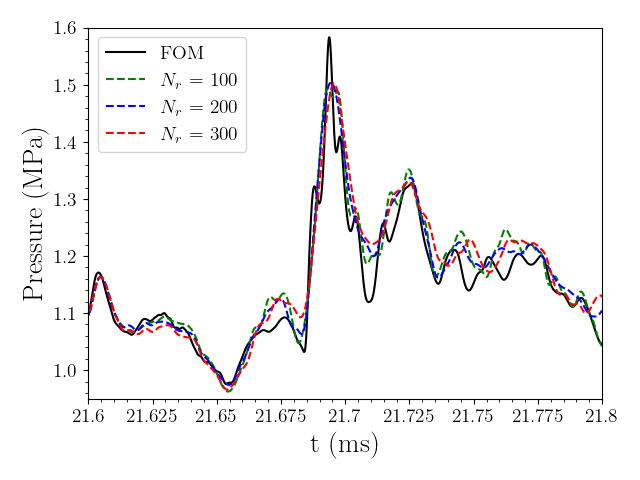
\includegraphics[width=0.99\linewidth]{Chapters/HPROMResults/Images/nineElem/deim/pressure_probe_deim_random_modes.png}
		\caption{\label{fig:nineElemDEIMProbeModes}Nine-element combustor HPPROM pressure probe measurements, random sampling, $\numSamps = 0.1\% \times \numDOF$ various $\numResModes$.}
	\end{minipage}
	\begin{minipage}{0.49\linewidth}
		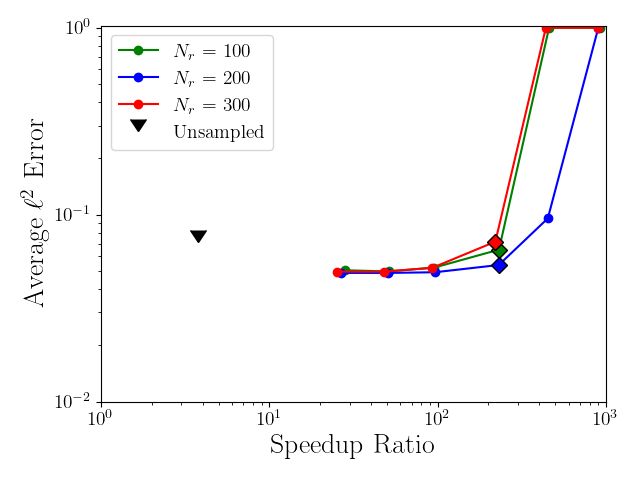
\includegraphics[width=0.99\linewidth]{Chapters/HPROMResults/Images/nineElem/deim/sampled_dt5e-7_Average_errorRaw_pareto.png}
		\caption{\label{fig:nineElemPareto}Nine-element combustor HPROM time-average error vs. CPU-time speedup, various $\numResModes$.}
	\end{minipage}
\end{figure}

The effect of the gappy POD regressor basis is noted by probe measurements in Fig.~\ref{fig:nineElemDEIMProbeModes}. To the human eye, there is little significant difference in the reconstruction of the pressure signal, implying a less significant effect of $\numResModes$ for this system than was observed for the cavity and CVRC cases. Aggregate error measurements, displayed with respect to computational cost speedup in Fig.~\ref{fig:nineElemPareto}, reveal similarly small discrepancies with regard to $\numResModes$. Unfortunately, as observed with the cavity and CVRC case, the random sampling algorithm is unable to generate the enormous cost savings and robust solutions that the eigenvector-based sampling was capable of for those cases. As the greedy algorithms appeared generally unstable, the random algorithm is able to produce, at best, roughly two orders of magnitude computational cost savings while remaining stable and accurate. Although not as impressive as the three to four orders of magnitude speedup observed for the CVRC case, this still represents a major accomplishment in the application of these methods to a problem of such high dimensionality and extreme physical complexity. Further, it serves as a testament to the ability of the MP-LSVT framework to generate accurate and robust solutions in combination with good computational cost savings when paired with a careful hyper-reduction approach.